\documentclass[utf8x, a4paper, 12pt, oneside]{extarticle}

\usepackage[utf8x]{inputenc}
\usepackage[english,russian]{babel}
\usepackage{shellesc}
\usepackage{amssymb,amsfonts,amsmath,mathtext,enumerate,float}
\usepackage{pgfplots}
\usepackage{graphicx}
\usepackage{svg}
\usepackage[off]{svg-extract}
\svgsetup{clean=true}
\usepackage{tocloft}
\usepackage{listings}
\usepackage{caption}
\usepackage{titlesec}
\usepackage{tempora}
\usepackage{setspace}
\usepackage[
  left=30mm,
  right=10mm,
  top=20mm,
  bottom=20mm,
  reversemp, % tell geometry marginpars are on the left
  marginparwidth=26mm, % width for the todo notes area
  marginparsep=3mm % gap between text block and margin note
]{geometry}
\usepackage{indentfirst}
\usepackage{pdfpages}
\usepackage{enumerate,letltxmacro}
\usepackage{threeparttable}
\usepackage[hidelinks]{hyperref}
\usepackage{flafter}
\usepackage{enumitem}
\usepackage{multirow}
\usepackage{longtable}
\usepackage[toc]{appendix}
\usepackage{wrapfig}
\usepackage{zref-totpages}

\usepackage{todonotes}
\usepackage{lastpage}

\usepackage{csquotes}

\usepackage[backend=biber,sorting=none,style=gost-numeric]{biblatex}
\addbibresource{sources.bib}

\usepackage[figure,table,equation]{totalcount}

\newcounter{totfigures}
\newcounter{tottables}
\newcounter{totequations}
\newcounter{totlistings}

\providecommand\totfig{} 
\providecommand\tottab{}
\providecommand\toteq{}

\pretocmd{\chapter}{\addtocounter{totfigures}{\value{figure}}\setcounter{figure}{0}}{}{}
\pretocmd{\chapter}{\addtocounter{tottables}{\value{table}}\setcounter{table}{0}}{}{}
\pretocmd{\chapter}{\addtocounter{totequations}{\value{equation}}\setcounter{equation}{0}}{}{}

\makeatletter
\AtEndDocument{%
  \addtocounter{totfigures}{\value{figure}}%
  \addtocounter{tottables}{\value{table}}%
  \addtocounter{totequations}{\value{equation}}%
  \immediate\write\@mainaux{%
    \string\gdef\string\totfig{\number\value{totfigures}}%
    \string\gdef\string\tottab{\number\value{tottables}}%
    \string\gdef\string\toteq{\number\value{totequations}}%
  }%
}
\makeatother

\makeatletter
\if@todonotes@disabled
\newcommand{\hlfix}[2]{#1}
\else
\newcommand{\hlfix}[2]{\texthl{#1}\todo{#2}}
\fi
\makeatother

\setlist{nosep}

\newcommand{\ssr}[1]{%
  \par\begingroup
    \centering\LARGE\bfseries #1\par
  \endgroup
  \phantomsection% важно, если есть hyperref
  \addcontentsline{toc}{section}{#1}%
}

\newcommand{\sssr}[1]{%
  \par\begingroup
    \centering\Large\bfseries #1\par
  \endgroup
  \phantomsection% важно, если есть hyperref
  \addcontentsline{toc}{section}{#1}%
}

\newcommand{\ssssr}[1]{%
	\par\begingroup
	\centering\large\bfseries #1\par
	\endgroup
	\phantomsection% важно, если есть hyperref
	\addcontentsline{toc}{section}{#1}%
}

\makeatletter
\renewcommand\LARGE{\@setfontsize\LARGE{22pt}{20}}
\renewcommand\Large{\@setfontsize\Large{20pt}{20}}
\renewcommand\large{\@setfontsize\large{16pt}{20}}
\makeatother
\RequirePackage{titlesec}
\titleformat{\chapter}[block]{\hspace{\parindent}\large\bfseries}{\thechapter}{0.5em}{\large\bfseries\raggedright}
\titleformat{name=\chapter,numberless}[block]{\hspace{\parindent}}{}{0pt}{\large\bfseries\centering}
\titleformat{\section}[block]{\hspace{\parindent}\large\bfseries}{\thesection}{0.5em}{\large\bfseries\raggedright}
\titleformat{\subsection}[block]{\hspace{\parindent}\large\bfseries}{\thesubsection}{0.5em}{\large\bfseries\raggedright}
\titleformat{\subsubsection}[block]{\hspace{\parindent}\large\bfseries}{\thesubsection}{0.5em}{\large\bfseries\raggedright}
\titlespacing{\chapter}{12.5mm}{-22pt}{10pt}
\titlespacing{\section}{12.5mm}{10pt}{10pt}
\titlespacing{\subsection}{12.5mm}{10pt}{10pt}
\titlespacing{\subsubsection}{12.5mm}{10pt}{10pt}

\makeatletter
\renewcommand{\@biblabel}[1]{#1.}
\makeatother
%
%\titleformat{\chapter}[hang]{\LARGE\bfseries}{\hspace{1.25cm}\thechapter}{1ex}{\LARGE\bfseries}
%\titleformat{\section}[hang]{\Large\bfseries}{\hspace{1.25cm}\thesection}{1ex}{\Large\bfseries}
%\titleformat{name=\section,numberless}[hang]{\Large\bfseries}{\hspace{1.25cm}}{0pt}{\Large\bfseries}
%\titleformat{\subsection}[hang]{\large\bfseries}{\hspace{1.25cm}\thesubsection}{1ex}{\large\bfseries}
%\titlespacing{\chapter}{0pt}{-\baselineskip}{\baselineskip}
%\titlespacing*{\section}{0pt}{\baselineskip}{\baselineskip}
%\titlespacing*{\subsection}{0pt}{\baselineskip}{\baselineskip}
\onehalfspacing

\renewcommand{\theenumi}{\arabic{enumi}}
\renewcommand{\labelenumi}{\arabic{enumi}\text{)}}
\renewcommand{\theenumii}{.\arabic{enumii}}
\renewcommand{\labelenumii}{\asbuk{enumii}\text{)}}
\renewcommand{\theenumiii}{.\arabic{enumiii}}
\renewcommand{\labelenumiii}{\arabic{enumi}.\arabic{enumii}.\arabic{enumiii}.}

%\renewcommand{\cftchapleader}{\cftdotfill{\cftdotsep}}
\renewcommand{\cftsecleader}{\cftdotfill{\cftdotsep}}
\renewcommand{\cftsubsecleader}{\cftdotfill{\cftdotsep}}
\renewcommand{\cftsubsubsecleader}{\cftdotfill{\cftdotsep}}


\addto\captionsrussian{\renewcommand{\figurename}{Рисунок}}
\DeclareCaptionLabelSeparator{dash}{~---~}
\captionsetup{labelsep=dash}

\DeclareCaptionFormat{fmt}{\parbox{\linewidth}{#1#2#3}}
\captionsetup{justification=raggedleft,format=fmt,position=bottom}
\captionsetup[figure]{justification=centering,format=default,labelsep=dash}

\graphicspath{{img/}}%путь к рисункам

\newcommand{\floor}[1]{\lfloor #1 \rfloor}

\lstset{ %
	language=python,                 % выбор языка для подсветки
	basicstyle=\small\sffamily, % размер и начертание шрифта для подсветки кода
	numbers=none,               % где поставить нумерацию строк (слева\справа)
	numberstyle=\tiny,           % размер шрифта для номеров строк
	stepnumber=1,                   % размер шага между двумя номерами строк
%	numbersep=5pt,                % как далеко отстоят номера строк от подсвечиваемого кода
	showspaces=false,            % показывать или нет пробелы специальными отступами
	showstringspaces=false,      % показывать или нет пробелы в строках
	showtabs=false,             % показывать или нет табуляцию в строках
	frame=single,              % рисовать рамку вокруг кода
	tabsize=2,                 % размер табуляции по умолчанию равен 2 пробелам
	captionpos=t,              % позиция заголовка вверху [t] или внизу [b] 
	breaklines=true,           % автоматически переносить строки (да\нет)
	breakatwhitespace=false, % переносить строки только если есть пробел
	escapeinside={\#*}{*)},   % если нужно добавить комментарии в коде
	abovecaptionskip=-5pt
}

\pgfplotsset{width=0.85\linewidth, height=0.5\columnwidth}

\linespread{1.3}

\parindent=1.25cm

%\LetLtxMacro\itemold\item
%\renewcommand{\item}{\itemindent0.75cm\itemold}

\def\labelitemi{---}
\setlist[itemize]{leftmargin=1.25cm, itemindent=0.65cm}
\setlist[enumerate]{leftmargin=1.25cm, itemindent=0.55cm}

\newcommand{\specialcell}[2][c]{%
	\begin{tabular}[#1]{@{}c@{}}#2\end{tabular}}

\frenchspacing

\lstset{
	literate=
	{а}{{\selectfont\char224}}1
	{б}{{\selectfont\char225}}1
	{в}{{\selectfont\char226}}1
	{г}{{\selectfont\char227}}1
	{д}{{\selectfont\char228}}1
	{е}{{\selectfont\char229}}1
	{ё}{{\"e}}1
	{ж}{{\selectfont\char230}}1
	{з}{{\selectfont\char231}}1
	{и}{{\selectfont\char232}}1
	{й}{{\selectfont\char233}}1
	{к}{{\selectfont\char234}}1
	{л}{{\selectfont\char235}}1
	{м}{{\selectfont\char236}}1
	{н}{{\selectfont\char237}}1
	{о}{{\selectfont\char238}}1
	{п}{{\selectfont\char239}}1
	{р}{{\selectfont\char240}}1
	{с}{{\selectfont\char241}}1
	{т}{{\selectfont\char242}}1
	{у}{{\selectfont\char243}}1
	{ф}{{\selectfont\char244}}1
	{х}{{\selectfont\char245}}1
	{ц}{{\selectfont\char246}}1
	{ч}{{\selectfont\char247}}1
	{ш}{{\selectfont\char248}}1
	{щ}{{\selectfont\char249}}1
	{ъ}{{\selectfont\char250}}1
	{ы}{{\selectfont\char251}}1
	{ь}{{\selectfont\char252}}1
	{э}{{\selectfont\char253}}1
	{ю}{{\selectfont\char254}}1
	{я}{{\selectfont\char255}}1
	{А}{{\selectfont\char192}}1
	{Б}{{\selectfont\char193}}1
	{В}{{\selectfont\char194}}1
	{Г}{{\selectfont\char195}}1
	{Д}{{\selectfont\char196}}1
	{Е}{{\selectfont\char197}}1
	{Ё}{{\"E}}1
	{Ж}{{\selectfont\char198}}1
	{З}{{\selectfont\char199}}1
	{И}{{\selectfont\char200}}1
	{Й}{{\selectfont\char201}}1
	{К}{{\selectfont\char202}}1
	{Л}{{\selectfont\char203}}1
	{М}{{\selectfont\char204}}1
	{Н}{{\selectfont\char205}}1
	{О}{{\selectfont\char206}}1
	{П}{{\selectfont\char207}}1
	{Р}{{\selectfont\char208}}1
	{С}{{\selectfont\char209}}1
	{Т}{{\selectfont\char210}}1
	{У}{{\selectfont\char211}}1
	{Ф}{{\selectfont\char212}}1
	{Х}{{\selectfont\char213}}1
	{Ц}{{\selectfont\char214}}1
	{Ч}{{\selectfont\char215}}1
	{Ш}{{\selectfont\char216}}1
	{Щ}{{\selectfont\char217}}1
	{Ъ}{{\selectfont\char218}}1
	{Ы}{{\selectfont\char219}}1
	{Ь}{{\selectfont\char220}}1
	{Э}{{\selectfont\char221}}1
	{Ю}{{\selectfont\char222}}1
	{Я}{{\selectfont\char223}}1
}


\begin{document}

\includepdf[pages={1,2}]{parts/title}

\ssr{РЕФЕРАТ}

Расчетно-пояснительная записка $\text{\ztotpages}$ с., \totfig\ рис., 24 ист.

ОПЕРАЦИОННЫЕ СИСТЕМЫ, ЗАГРУЖАЕМЫЙ МОДУЛЬ ЯДРА, ПОДСИСТЕМА ВВОДА, BLUETOOTH, RFCOMM, ВИРТУАЛЬНОЕ УСТРОЙСТВО МЫШИ

Цель работы — разработка загружаемого модуля ядра Linux, обеспечивающего управление курсором мыши с использованием сенсорного экрана мобильного устройства по каналу Bluetooth.

В работе реализовано виртуальное устройство ввода типа «мышь», зарегистрированное в подсистеме input ядра Linux. Передача управляющих данных осуществляется по протоколу RFCOMM. Мобильное приложение для операционной системы Android формирует сообщения о перемещении курсора и состояниях кнопок мыши на основе событий сенсорного экрана.

Разработанный модуль обеспечивает приём сообщений по Bluetooth, их декодирование и генерацию соответствующих событий подсистемы ввода. Реализованное программное решение позволяет использовать мобильное устройство в качестве беспроводного манипулятора для управления курсором рабочей станции.

\pagebreak


\begingroup
  \renewcommand{\addvspace}[1]{}% убрать вертикальные отступы внутри оглавления
  \renewcommand{\contentsname}{\begin{center}СОДЕРЖАНИЕ\end{center}}
  \tableofcontents
\endgroup

\ssr{СОКРАЩЕНИЯ}

HID --- Human Interface Device

RFCOMM --- Radio Frequency Communication


\ssr{ВВЕДЕНИЕ}

% Операционные системы на базе ядра Linux широко применяются на серверных, настольных и встраиваемых платформах, в том числе в составе мобильных операционных систем и специализированных дистрибутивов для рабочих станций и ноутбуков~\cite{stackoverflow-survey-2024}. Расширение функциональности ядра осуществляется с помощью загружаемых модулей, которые интегрируются в существующие подсистемы ввода-вывода и сетевого стека без пересборки ядра \cite{linux-driver-basics}.

% Цель работы --- разработка загружаемого модуля ядра Linux, реализующего виртуальное устройство мыши, и сопряжённого мобильного приложения на базе Android, обеспечивающих управление курсором рабочей станции по каналу Bluetooth с использованием сенсорного экрана телефона.

% Для достижения поставленной цели требуется решить следующие задачи:
% \begin{enumerate}
% 	\item провести анализ способов управления курсором мыши из загружаемого модуля ядра;
% 	\item провести анализ способов взаимодействия между телефоном и загружаемым модулем ядра;
% 	\item реализовать алгоритмы, загружаемый модуль ядра Linux и Android приложение для управления курсором мыши с помощью сенсорного экрана телефона.
% \end{enumerate}

Использование беспроводных устройств ввода является актуальной задачей в области операционных систем и встроенного программного обеспечения. Управление курсором с помощью мобильного устройства позволяет расширить возможности взаимодействия пользователя с рабочей станцией без применения специализированных аппаратных манипуляторов.

В данной работе разрабатывается загружаемый модуль ядра Linux, реализующий виртуальное устройство ввода типа «мышь», управление которым осуществляется с использованием сенсорного экрана мобильного телефона по каналу Bluetooth. Для формирования управляющих воздействий используется мобильное приложение под управлением операционной системы Android.

Целью работы является разработка загружаемого модуля ядра Linux и сопряжённого мобильного приложения, обеспечивающих передачу команд управления курсором от мобильного устройства к рабочей станции по беспроводному каналу связи.

Для достижения поставленной цели необходимо выполнить следующие задачи:
\begin{itemize}
	\item провести анализ способов управления курсором мыши из загружаемого модуля ядра Linux;
	\item провести анализ способов обмена данными между мобильным устройством и модулем ядра по каналу Bluetooth;
	\item разработать алгоритмы функционирования загружаемого модуля ядра и мобильного приложения;
	\item реализовать загружаемый модуль ядра Linux, обеспечивающий генерацию событий подсистемы ввода;
	\item реализовать мобильное приложение для операционной системы Android;
	\item выполнить тестирование разработанного программного комплекса.
\end{itemize}


\section{Аналитический раздел}

\subsection{Постановка задачи}

В соответствии с заданием на курсовую работу, необходимо разработать загружаемый модуль ядра Linux, реализующий виртуальное устройство мыши, принимающий команды от мобильного приложения на смартфоне по каналу Bluetooth и преобразующий эти команды в события подсистемы ввода.

Для выполнения этой задачи требуется:
\begin{enumerate}
	\item проанализировать предметную область;
	\item разработать алгоритмы и структуру загружаемого модуля ядра, обрабатывающего информацию, полученную со смартфона и преобразующего её в события подсистемы ввода;
	\item реализовать загружаемый модуль ядра, выполняющий поставленную задачу;
	\item протестировать работу реализованного загружаемого модуля ядра.
\end{enumerate}

\subsection{Анализ способов преобразования касаний сенсорного экрана в перемещение курсора мыши}

При интеграции мобильного приложения, формирующего события касаний, и загружаемого модуля ядра, эмулирующего поведение мыши, необходимо определить способ сопоставления данных сенсорного экрана с координатами курсора.

В соответствии с логикой построения указательных устройств рассмотрены два подхода:
\begin{enumerate}
\item преобразование координат касаний в \textit{абсолютные} координаты на экране ПК;
\item преобразование перемещения пальца в \textit{относительные} смещения курсора.
\end{enumerate}

Абсолютные координаты требуют точного соответствия геометрии сенсорного устройства и рабочего стола, а также нормализации значений, поступающих от Android-приложения, к диапазону координат подсистемы ввода ядра Linux. Такой способ приводит к ряду ограничений: несовпадение пропорций сенсорной панели и монитора, масштабирование рабочего стола и наличие нескольких экранов приводят к неоднозначности отображения координат. 

Абсолютное позиционирование предполагает передачу полного набора координат при каждом событии касания, что повышает интенсивность обмена данными по Bluetooth и увеличивает требования к стабильности канала связи.

Использование относительных координат основано на передаче смещений \textit{dx, dy}, вычисляемых из последовательности касаний (или непрерывного перемещения пальца). 
Такой подход соответствует модели классических компьютерных мышей, где устройство генерирует относительные изменения положения независимо от абсолютной позиции курсора. 

Кроме того, относительные смещения естественным образом интегрируются в архитектуру Android-приложения, где компонент обработчика касаний оперирует разностями координат, что исключает необходимость приведения значений к масштабу удалённого экрана.

С учётом перечисленных факторов, был выбран способ передачи \textit{относительных координат}. 
Он достаточен для обеспечения перемещения курсора мыши и не требует конфигурации для сопоставления масштабов экрана.


\subsection{Способы обмена данными между телефоном и модулем ядра}

Передача данных между мобильным устройством и загружаемым модулем ядра может быть реализована различными способами, включая сетевые протоколы, каналы межпроцессного взаимодействия через пользовательское пространство и беспроводные стеки передачи данных.

Для решения поставленной задачи выбрано беспроводное соединение по технологии Bluetooth. Оно обеспечивает устойчивый двунаправленный канал связи, нативно поддерживается в ядре Linux через подсистему \texttt{BlueZ} и предоставляет API, совместимый с типовыми средствами разработки Android-приложений.

Стек Bluetooth в Linux реализуется в виде подсистемы \texttt{BlueZ}, включающей поддержку базового протокола L2CAP, протокола RFCOMM, профиля HID и вспомогательных служб~\cite{bluetooth-core-spec,bluez-l2cap-wiki,bluez-rfcomm-wiki}. На уровне ядра для взаимодействия с Bluetooth-устройствами используются сокеты семейства \texttt{PF\_BLUETOOTH} с такими протоколами, как \texttt{BTPROTO\_L2CAP} и \texttt{BTPROTO\_RFCOMM}~\cite{bluetooth-core-spec,kernel-net-kapi}. В пространстве ядра доступен интерфейс для создания и использования таких сокетов, обеспечивающий работу с Bluetooth-соединениями без участия пользовательского процесса~\cite{kernel-net-kapi}.

С точки зрения обмена данными между смартфоном и модулем ядра возможны следующие варианты:
\begin{enumerate}
	\item использование RFCOMM-сокетов в пространстве ядра;
	\item работа непосредственно с L2CAP в пространстве ядра;
	\item задействование профиля HID поверх Bluetooth;
	\item использование устройств \texttt{/dev/rfcommN} и пользовательского пространства.
\end{enumerate}

\

\textit{RFCOMM-сокеты в пространстве ядра}

Протокол RFCOMM реализует поверх L2CAP байтовый поток, логически аналогичный последовательному порту, и применяется для построения сервисов, требующих надёжного двунаправленного канала~\cite{bluetooth-core-spec,bluez-rfcomm-wiki}. В ядре Linux поддержка RFCOMM интегрирована в сетевой стек, что позволяет создавать серверные и клиентские сокеты с использованием семейства \texttt{PF\_BLUETOOTH} и протокола \texttt{BTPROTO\_RFCOMM}~\cite{bluetooth-core-spec,linux-rfcomm-core}. Адресация RFCOMM-сокета выполняется с использованием структуры адреса, содержащей семейство, Bluetooth-адрес удалённого устройства и номер канала.

На стороне Android-приложения подключение к такому сервису реализуется через API класса \texttt{BluetoothSocket}, который инкапсулирует установление RFCOMM-соединения по указанному UUID сервиса~\cite{android-bt-connect,BluetoothSocket-doc}. Таким образом реализуется связка: серверный RFCOMM-сокет в пространстве ядра и клиентское соединение в приложении Android.

При использовании RFCOMM модуль ядра получает поток байтов непосредственно от смартфона, что позволяет задать прикладной протокол управления курсором (например, фиксированный формат кадров с координатами и битовой маской кнопок) без вовлечения дополнительных уровней абстракции~\cite{bluetooth-core-spec,bluez-rfcomm-wiki}. Обработка входящего потока выполняется в  обработчиках на стороне загружаемого модуля ядра, что упрощает синхронизацию с подсистемой ввода~\cite{kernel-net-kapi}.

\

\textit{Использование L2CAP в пространстве ядра}

L2CAP представляет собой базовый протокол Bluetooth, обеспечивающий мультиплексирование каналов и передачу пакетов между устройствами~\cite{bluetooth-core-spec,bluez-l2cap-wiki}. Прямое использование L2CAP даёт доступ к более низкому уровню стека и предоставляет гибкость при реализации собственных протоколов, но требует дополнительной обработки параметров канала и управления MTU~\cite{l2cap-man}.

В контексте рассматриваемой задачи использование L2CAP в качестве средства передачи данных для прикладного протокола управления курсором приводит к усложнению логики модуля ядра и дублированию функциональности, уже реализованной в RFCOMM, как надстройке над L2CAP~\cite{bluetooth-core-spec,bluez-l2cap-wiki}.
Кроме того, на стороне Android типовые высокоуровневые API ориентированы на RFCOMM-сервисы, что делает прямую работу с L2CAP при реализации мобильного приложения неоправданным ограничением~\cite{android-bt-connect}.

\

\textit{Профиль HID поверх Bluetooth}

Для устройств ввода, Bluetooth-стек предусматривает профиль HID, обеспечивающий транспорт HID-отчётов по каналу L2CAP и интеграцию с HID-core ядра~\cite{bluetooth-core-spec,linux-hid-docs}. Такой подход используется для аппаратных Bluetooth-мышей и клавиатур: транспортный драйвер профиля HID принимает HID-отчёты по Bluetooth и передаёт их в HID-core, где они интерпретируются и преобразуются в события подсистемы ввода~\cite{linux-hid-docs,hidp-core-doc}. Поддержка профиля HIDP на стороне ядра конфигурируется параметром \texttt{CONFIG\_BT\_HIDP} в конфигурации ядра~\cite{config-bt-hidp}.

Применение профиля HID для эмуляции мыши на базе смартфона потребовало бы разработки или адаптации транспортного драйвера, а также формирования корректных HID-описателей и отчётов~\cite{hid-transport,hidintro}. В рамках курсовой работы такая интеграция выходит за пределы необходимого объёма, так как влечёт за собой разработку HID-описателя, поддержку отчётов и согласование с существующей инфраструктурой HID при отсутствии требований к использованию расширенных возможностей HID-протокола~\cite{linux-hid-docs,hiddev-doc}.

\

\textit{Использование устройств \texorpdfstring{\texttt{/dev/rfcommN}}{dev/rfcommN} и пользовательского пространства}

Подсистема \texttt{BlueZ} предоставляет возможность отображать RFCOMM-соединения в виде псевдотерминальных устройств \texttt{/dev/rfcommN}, которые доступны пользовательским приложениям как последовательные порты~\cite{bluez-rfcomm-wiki,rfcomm-tty-howto}. Пользовательские программы открывают такие устройства через стандартные системные вызовы и читают поток байтов, реализуя прикладной протокол в пользовательском пространстве~\cite{rfcomm-tty-howto,rfcomm-missing-dev}.

Для интеграции с модулем ядра в этом случае потребовалась бы дополнительная связка между пользовательским процессом, обрабатывающим \texttt{/dev/rfcommN}, и драйвером мыши, например через символьное устройство или вспомогательный интерфейс обмена. Такая архитектура приводит к разделению логики между модулем ядра и пользовательским процессом и увеличивает количество точек отказа. Кроме того, основной функциональный поток управления курсором в этом случае реализуется в пользовательском пространстве, тогда как модуль ядра выполняет вспомогательные функции маршрутизации событий~\cite{linux-driver-basics}.

\

\textit{Обоснование выбора RFCOMM-сокета в пространстве ядра}

В результате анализа способов передачи данных в модуль ядра по протоколу Bluetooth, получены следующие выводы:
\begin{itemize}
	\item L2CAP предоставляет универсальный транспортный уровень и используется в качестве основы для протоколов более высокого уровня, однако при прямом использовании влечёт усложнение драйвера за счёт необходимости дополнительной обработки параметров канала~\cite{bluetooth-core-spec,bluez-l2cap-wiki,l2cap-man};
	\item профиль HID ориентирован на аппаратные HID-устройства и предполагает интеграцию с HID-core и существующей реализацией профиля в ядре, что не требуется для протокола обмена фиксированного формата между смартфоном и драйвером мыши~\cite{bluetooth-core-spec,linux-hid-docs,hidp-core-doc,config-bt-hidp};
	\item использование \texttt{/dev/rfcommN} и пользовательских программ переводит основную часть обработки в пользовательское пространство и требует дополнительного канала взаимодействия с модулем ядра~\cite{bluez-rfcomm-wiki,rfcomm-tty-howto,linux-driver-basics};
	\item RFCOMM-сокет в пространстве ядра обеспечивает потоковый канал непосредственно в драйвер, использует реализованный протокол поверх L2CAP и поддерживает соединение с высокоуровневым API Android-приложения~\cite{linux-rfcomm-core,kernel-net-kapi,android-bt-connect,BluetoothSocket-doc}.
\end{itemize}

На основании этих соображений в разрабатываемом драйвере выбран подход, основанный на серверном RFCOMM-сокете в пространстве ядра. 
Модуль ядра, фактически, становится сервером, к которому присоединяются клиенты с помощью мобильного приложения Android.
Этот сервер обрабатывает сообщения фиксированного формата с данными о перемещении и состояниях кнопок, выполняет обработку входящих данных и синхронно генерирует события подсистемы ввода для виртуального устройства мыши~\cite{linux-input-docs,bluetooth-core-spec,android-bt-connect}. 
Такой стек (виртуальное устройство в подсистеме input и RFCOMM-соединение в пространстве ядра) соответствует постановке задачи и является достаточным для реализации драйвера.


\subsection{Анализ способов управления курсором мыши из загружаемого модуля ядра}

Для генерации событий подсистемы ввода рассмотрено два подхода: регистрация собственного виртуального устройства в подсистеме input и вмешательство в существующий стек ввода (перехват/модификация событий уже зарегистрированных устройств или графической подсистемы).

\

\textit{Виртуальное устройство в подсистеме input}

Этот способ заключается в регистрации виртуального устройства мыши через подсистему input~\cite{linux-input-docs,input-programming}. Модуль выделяет и инициализирует \texttt{struct input\_dev}, настраивает поддержку событий \texttt{EV\_REL} (\texttt{REL\_X}, \texttt{REL\_Y}) и \texttt{EV\_KEY} (\texttt{BTN\_LEFT}, \texttt{BTN\_RIGHT}), после чего регистрирует устройство в input-core~\cite{linux-input-docs}. Структура \texttt{input\_dev} и функции \texttt{input\_report\_*} объявлены в заголовочном файле \texttt{<linux/input.h>} ядра Linux. Генерация событий выполняется вызовами \texttt{input\_report\_rel}, \texttt{input\_report\_key} и \texttt{input\_sync}, что делает виртуальное устройство эквивалентным аппаратной мыши для остального стека ввода~\cite{linux-input-docs}.

Структура \texttt{struct input\_dev} приведена в листинге~\ref{lst:input_dev}.

\begin{lstlisting}[language=C,caption={Структура \texttt{input\_dev}},label={lst:input_dev}]
	struct input_dev {
		const char * name;
		const char * phys;
		const char * uniq;
		struct input_id id;
		unsigned long propbit;
		unsigned long evbit;
		unsigned long keybit;
		unsigned long relbit;
		unsigned long absbit;
		unsigned long mscbit;
		unsigned long ledbit;
		unsigned long sndbit;
		unsigned long ffbit;
		unsigned long swbit;
		unsigned int hint_events_per_packet;
		unsigned int keycodemax;
		unsigned int keycodesize;
		void * keycode;
		int (* setkeycode) (struct input_dev *dev,const struct input_keymap_entry *ke, unsigned int *old_keycode);
		int (* getkeycode) (struct input_dev *dev, struct input_keymap_entry *ke);
		struct ff_device * ff;
		unsigned int repeat_key;
		struct timer_list timer;
		int rep;
		struct input_mt * mt;
		struct input_absinfo * absinfo;
		unsigned long key;
		unsigned long led;
		unsigned long snd;
		unsigned long sw;
		int (* open) (struct input_dev *dev);
		void (* close) (struct input_dev *dev);
		int (* flush) (struct input_dev *dev, struct file *file);
		int (* event) (struct input_dev *dev, unsigned int type, unsigned int code, int value);
		struct input_handle __rcu * grab;
		spinlock_t event_lock;
		struct mutex mutex;
		unsigned int users;
		bool going_away;
		struct device dev;
		struct list_head h_list;
		struct list_head node;
		unsigned int num_vals;
		unsigned int max_vals;
		struct input_value * vals;
		bool devres_managed;
	};
\end{lstlisting}

\

\textit{Перехват или модификация существующего стека ввода}

Альтернативный вариант — вмешательство в уже зарегистрированные устройства или обработчики графической подсистемы (например, перехват операций \lstinline|/dev/input/eventX|, модификация обработчиков оконной системы). Такой подход требует изменения существующих компонентов стека ввода или добавления промежуточных слоёв, усложняет сопровождение и увеличивает количество точек отказа. Кроме того, он не создаёт самостоятельного модуля ядра для эмуляции мыши, что расходится с задачей разработки отдельного загружаемого модуля.


\subsection{Минимальные структуры и точки входа модуля}

Загружаемый модуль ядра использует следующие точки входа~\cite{linux-driver-basics}:
\begin{itemize}
	\item функцию инициализации, регистрируемую через макрос \lstinline|module_init| (объявлен в \texttt{<linux/init.h>}), выполняющую создание виртуального устройства ввода, настройку RFCOMM-сокета и запуск служебного потока;
	\item функцию завершения, регистрируемую через макрос \lstinline|module_exit| из \texttt{<linux/init.h>}, выполняющую остановку служебного потока, закрытие RFCOMM-сокета и снятие виртуального устройства с регистрации в подсистеме ввода;
	\item функцию служебного потока обработки соединения, создаваемого с помощью \lstinline|kthread_run| (объявлена в \texttt{<linux/kthread.h>}) и выполняющего цикл приёма команд по RFCOMM и генерацию событий ввода~\cite{linux-kthread-man}.
\end{itemize}

Для интеграции с подсистемой ввода используется структура \lstinline|struct input_dev|, в которой настраиваются:
\begin{itemize}
	\item поддерживаемые типы событий \lstinline|EV_REL| и \lstinline|EV_KEY|;
	\item коды событий \lstinline|REL_X|, \lstinline|REL_Y|, \lstinline|BTN_LEFT|, \lstinline|BTN_RIGHT|;
	\item идентификаторы производителя, продукта и человекочитаемое имя устройства~\cite{linux-input-docs,input-programming}.
\end{itemize}
Генерация событий выполняется вызовами \lstinline|input_report_rel|, \lstinline|input_report_key| и \lstinline|input_sync| для зарегистрированного устройства~\cite{linux-input-docs}.

Для взаимодействия с RFCOMM создаётся серверный Bluetooth-сокет с семейством \lstinline|PF_BLUETOOTH| и протоколом \lstinline|BTPROTO_RFCOMM|. Адрес сокета задаётся структурой адреса с полями семейства адресов, Bluetooth-адреса устройства и номера RFCOMM-канала, после чего выполняются операции привязки и перевода сокета в режим прослушивания~\cite{bluetooth-core-spec,kernel-net-kapi,linux-rfcomm-core}.


\subsection*{Выводы}

Проанализированы способы сопоставления данных сенсорного экрана с перемещением курсора. 
Было рассмотрено использование абсолютных координат и относительных смещений \texttt{dx/dy}. 
Сравнительный анализ способов сопоставления данных сенсорного экрана с перемещением курсора приведён в таблице~\ref{tab:cursor-mapping-comparison}.

\begin{longtable}{|p{0.26\linewidth}|p{0.33\linewidth}|p{0.33\linewidth}|}
\caption{Сравнительный анализ способов сопоставления данных сенсорного экрана с перемещением курсора}\label{tab:cursor-mapping-comparison}\\
\hline
Критерий & Абсолютные координаты & Относительные смещения \\
\hline
Зависимость от геометрии экранов & Есть & Нет \\
\hline
Объём передаваемых данных & Полные координаты & Только смещения \texttt{dx/dy} \\
\hline
Устойчивость к многомониторным конфигурациям & Требуется нормализация и учёт топологии & Не требует специальных настроек \\
\hline
\end{longtable}

Был выбран способ передачи относительных смещений, так как этот подход независим от геометрии экранов, минимизирует объём данных и достаточен для перемещения курсора мыши.

\

Проанализированы способы удалённого взаимодействия устройств на основе подсистемы Bluetooth.
Было рассмотрено взаимодействие по протоколу L2CAP и использование RFCOMM в пространстве ядра. 
RFCOMM обеспечивает потоковый канал, прямо поддерживается Android API и не требует ручной сборки пакетов. 
Использование протокола L2CAP требует собственной обработки параметров канала и не имеет стандартной поддержки на стороне Android-приложения. 
Был выбран RFCOMM-сокет в пространстве ядра, так как он совместим с Android API и обеспечивает надёжный обмен без усложнения модуля.

\

Проанализированы способы генерации событий ввода. 
Была рассмотрена регистрация собственного \texttt{input\_dev} и вмешательство в существующий стек ввода.
Для \texttt{input\_dev} доступны прямые вызовы \texttt{input\_report\_*}, обеспечивающие полный контроль над формируемыми событиями в пределах модуля ядра.
Вмешательство в существующий стек зависит от внешних обработчиков и их форматов, что накладывает ограничения и увеличивает риск несовместимостей. 
Был выбран вариант с регистрацией собственного виртуального устройства ввода. 
Прямое формирование \texttt{EV\_REL}/\texttt{EV\_KEY} в модуле обеспечивает требуемый функционал без вмешательства в существующий стек ввода. 
Виртуальное устройство определяется системой как компьютерная мышь, что позволяет производить настраивать устройство в том числе и с помощью настроек графической оболочки системы.


\section{Конструкторский раздел}

\subsection{Общая структура решения}

Разрабатываемое решение включает два основных компонента:
\begin{itemize}
	\item загружаемый модуль ядра Linux, регистрирующий виртуальное устройство ввода типа «мышь» в подсистеме ввода и принимающий команды по RFCOMM-соединению Bluetooth~\cite{linux-input-docs,input-programming,bluetooth-core-spec,bluez-rfcomm-wiki};
	\item мобильное приложение для Android, устанавливающее RFCOMM-соединение с рабочей станцией и преобразующее действия пользователя на сенсорном экране в последовательность бинарных сообщений фиксированного формата~\cite{android-bt-connect,BluetoothSocket-doc}.
\end{itemize}

Модуль ядра взаимодействует с подсистемой ввода через структуру \lstinline|struct input_dev| и функции генерации событий ввода~\cite{linux-input-docs,input-programming}, а с подсистемой Bluetooth --- через серверный сокет с семейством \lstinline|PF_BLUETOOTH| и протоколом \lstinline|BTPROTO_RFCOMM|~\cite{bluetooth-core-spec,kernel-net-kapi,linux-rfcomm-core}. Мобильное приложение использует стек Bluetooth Android и API \lstinline|BluetoothAdapter|, \lstinline|BluetoothDevice| и \lstinline|BluetoothSocket| для установления соединения с модулем ядра и обмена бинарными сообщениями~\cite{android-bt-connect,BluetoothSocket-doc}.

\begin{figure}[h!]
	\centering
	\includegraphics[width=0.95\textwidth]{idef0.drawio.png}
	\caption{IDEF0-диаграмма подсистемы управления курсором с телефона}
	\label{fig:idef0}
\end{figure}
\clearpage

\subsection{Базовые структуры и точки входа драйвера}

Загружаемый модуль ядра использует следующие точки входа~\cite{linux-driver-basics}:
\begin{itemize}
	\item функцию инициализации, регистрируемую через макрос \lstinline|module_init|, выполняющую создание виртуального устройства ввода, настройку RFCOMM-сокета и запуск служебного потока;
	\item функцию завершения, регистрируемую через макрос \lstinline|module_exit|, выполняющую остановку служебного потока, закрытие RFCOMM-сокета и снятие виртуального устройства с регистрации в подсистеме ввода;
	\item функцию служебного потока обработки соединения, создаваемого с помощью \lstinline|kthread_run| и выполняющего цикл приёма команд по RFCOMM и генерацию событий ввода~\cite{linux-kthread-man}.
\end{itemize}

Для интеграции с подсистемой ввода используется структура \lstinline|struct input_dev|, в которой настраиваются:
\begin{itemize}
	\item поддерживаемые типы событий \lstinline|EV_REL| и \lstinline|EV_KEY|;
	\item коды событий \lstinline|REL_X|, \lstinline|REL_Y|, \lstinline|BTN_LEFT|, \lstinline|BTN_RIGHT|;
	\item идентификаторы производителя, продукта и человекочитаемое имя устройства~\cite{linux-input-docs,input-programming}.
\end{itemize}
Генерация событий выполняется вызовами \lstinline|input_report_rel|, \lstinline|input_report_key| и \lstinline|input_sync| для зарегистрированного устройства~\cite{linux-input-docs}.

Для взаимодействия с RFCOMM создаётся серверный Bluetooth-сокет с семейством \lstinline|PF_BLUETOOTH| и протоколом \lstinline|BTPROTO_RFCOMM|. Адрес сокета задаётся структурой адреса с полями семейства адресов, Bluetooth-адреса устройства и номера RFCOMM-канала, после чего выполняются операции привязки и перевода сокета в режим прослушивания~\cite{bluetooth-core-spec,kernel-net-kapi,linux-rfcomm-core}.

\subsection{Последовательность работы модуля ядра}

Работа модуля ядра логически разделяется на три этапа: инициализацию, обслуживание соединения и завершение работы.

На этапе инициализации выполняются проверка параметров, регистрация виртуального устройства ввода в подсистеме input, создание и настройка серверного RFCOMM-сокета и запуск служебного потока обработки соединения. Последовательность действий функции инициализации представлена на рис.~\ref{fig:module-load-scheme}.

\begin{figure}[h!]
	\centering
	\includegraphics[width=0.95\textwidth]{module_load_scheme.drawio.png}
	\caption{Схема алгоритма инициализации модуля ядра \texttt{phone\_mouse\_bt}}
	\label{fig:module-load-scheme}
\end{figure}
\clearpage

Служебный поток \lstinline|rx_loop| реализует цикл ожидания входящего RFCOMM-соединения, приёма и проверки сообщений фиксированной длины, обработки разрыва соединения и передачи декодированных команд во внутренние обработчики, генерирующие события ввода. Логика работы потока, включая обработку временного отсутствия данных, разрыва соединения и игнорирования некорректных пакетов, показана на рис.~\ref{fig:rx-loop-scheme}.
\begin{figure}[h!]
	\centering
	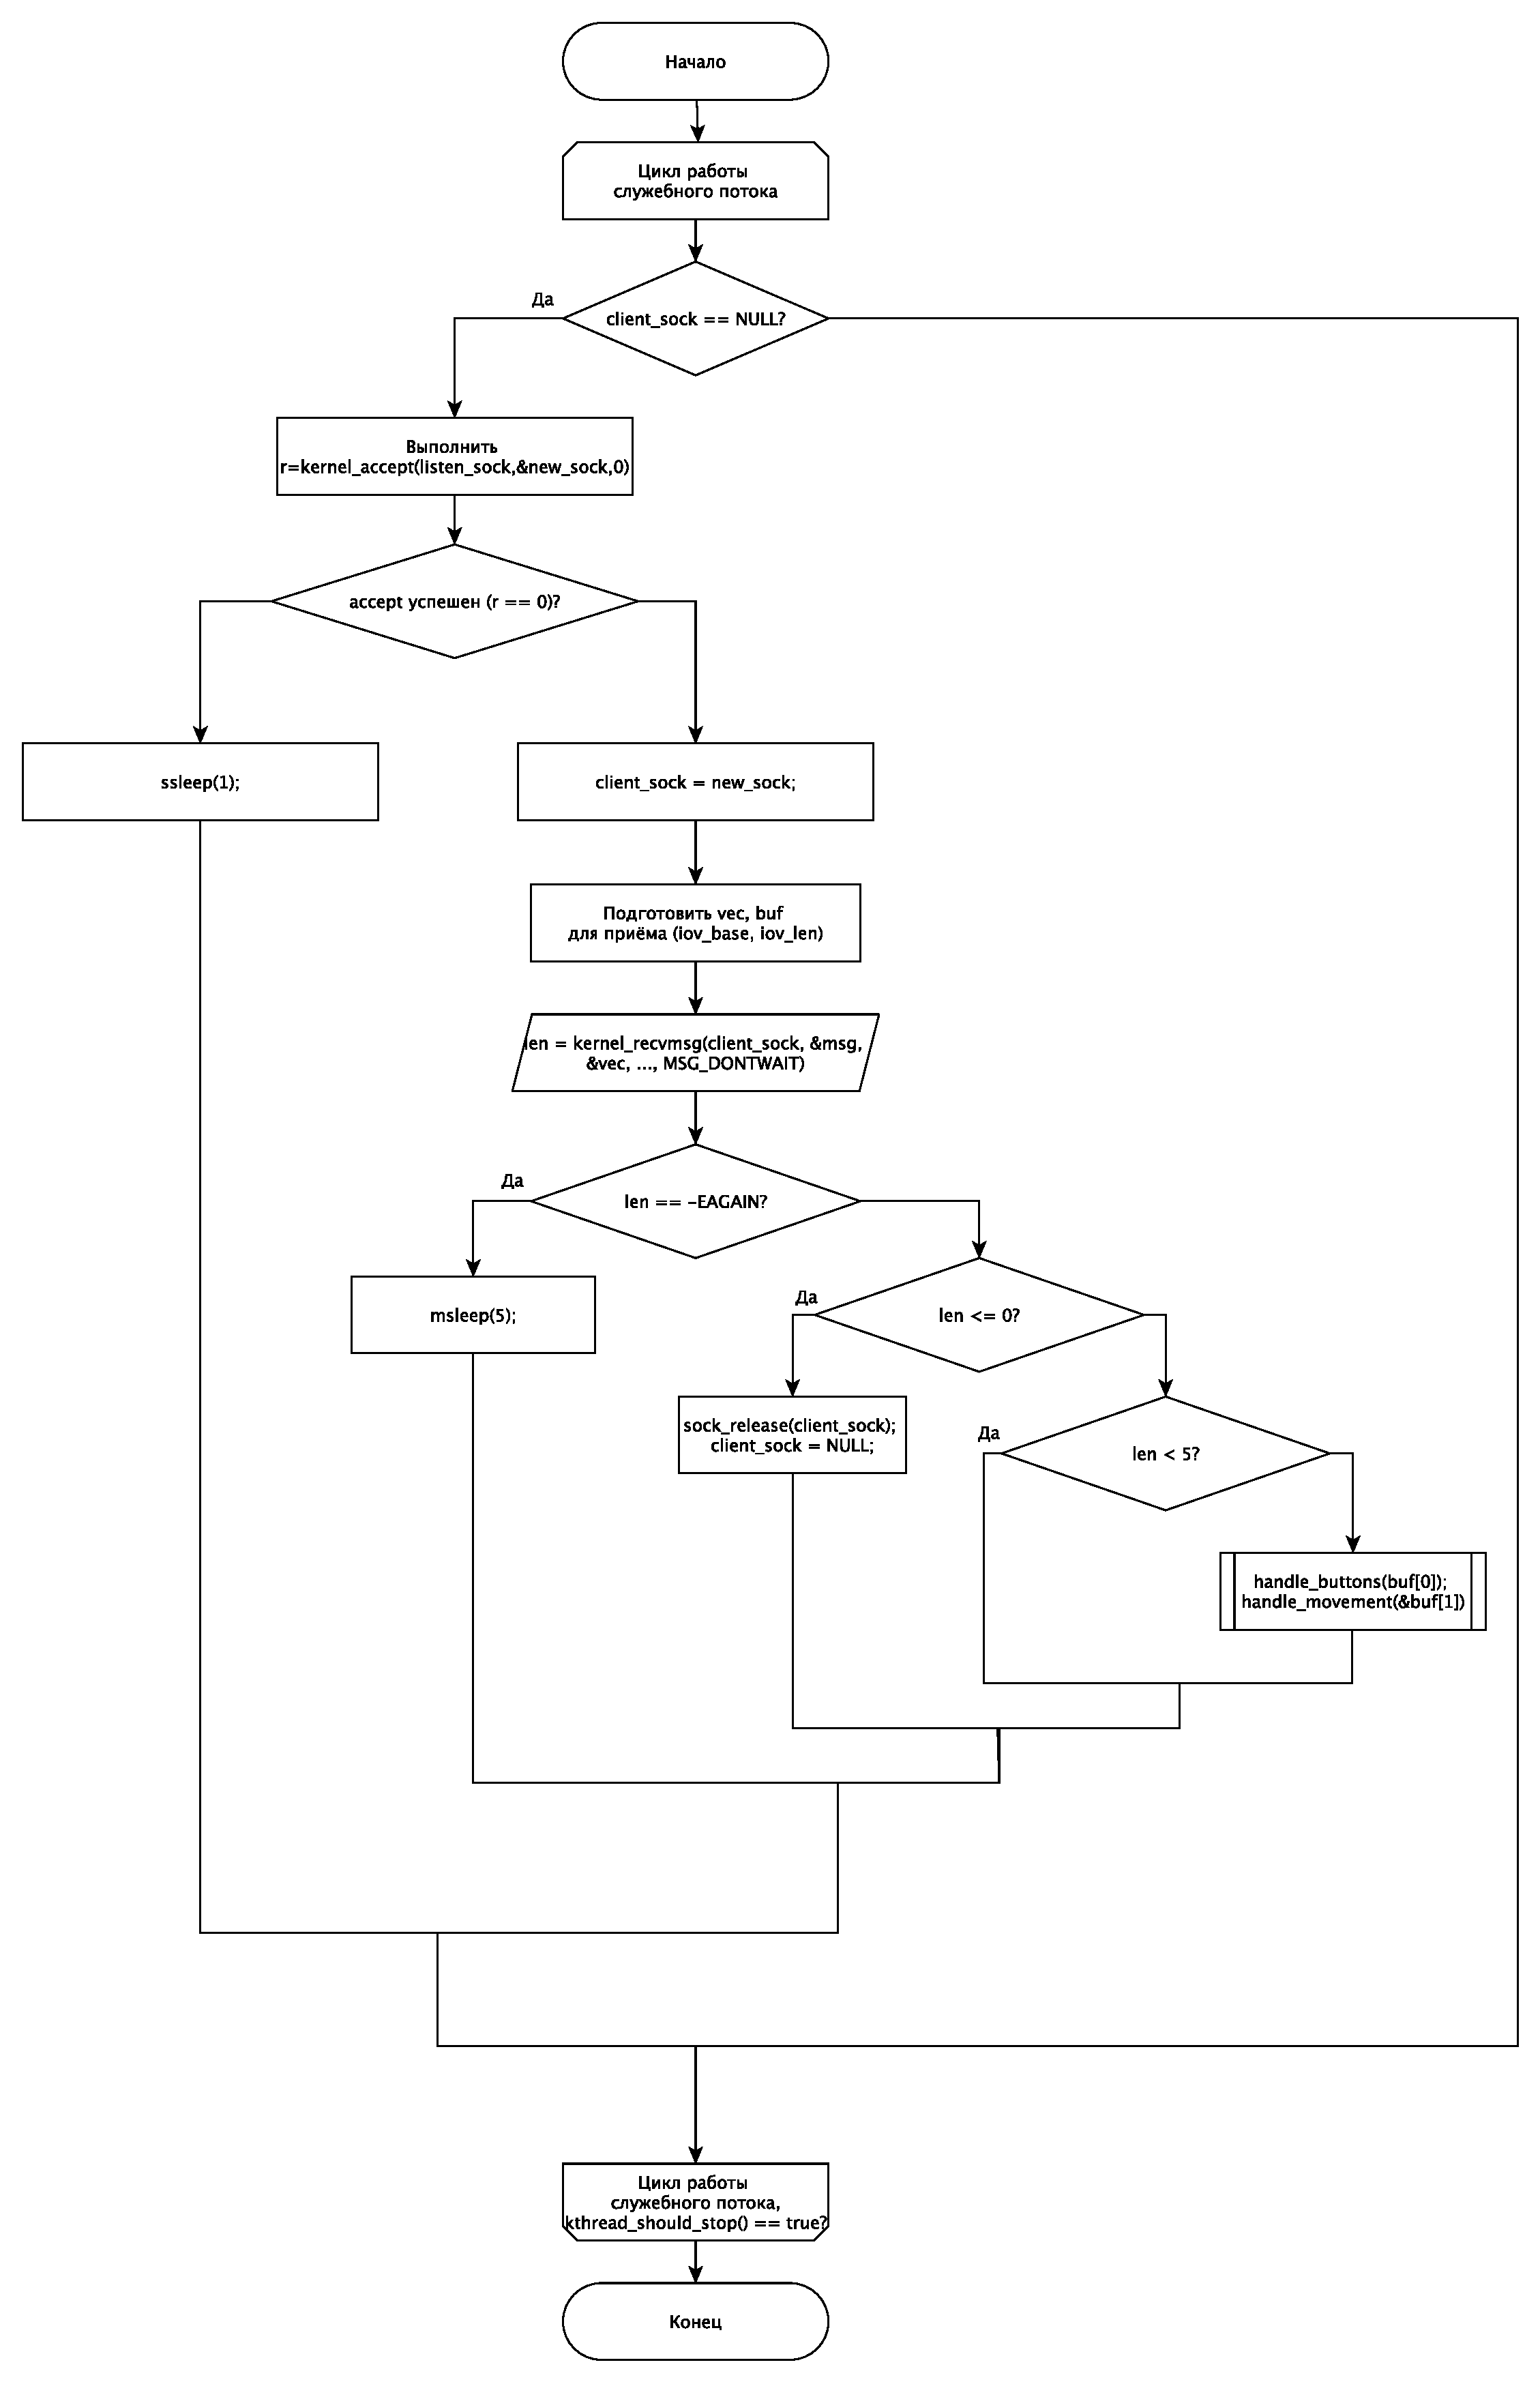
\includegraphics[height=0.7\textheight]{rx-loop.pdf}
	\caption{Схема алгоритма работы служебного потока \texttt{rx\_loop}}
	\label{fig:rx-loop-scheme}
\end{figure}
\clearpage

Обработка состояний кнопок мыши вынесена в отдельную функцию \lstinline|handle_buttons|. Эта функция декодирует битовую маску нажатых кнопок и порождает для каждой активной кнопки последовательность событий нажатия и отпускания с вызовами \lstinline|input_report_key| и \lstinline|input_sync|, формируя короткие клики левой и правой кнопок мыши. Схема алгоритма \lstinline|handle_buttons| приведена на рис.~\ref{fig:handle-buttons-scheme}.

\begin{figure}[h!]
	\centering
	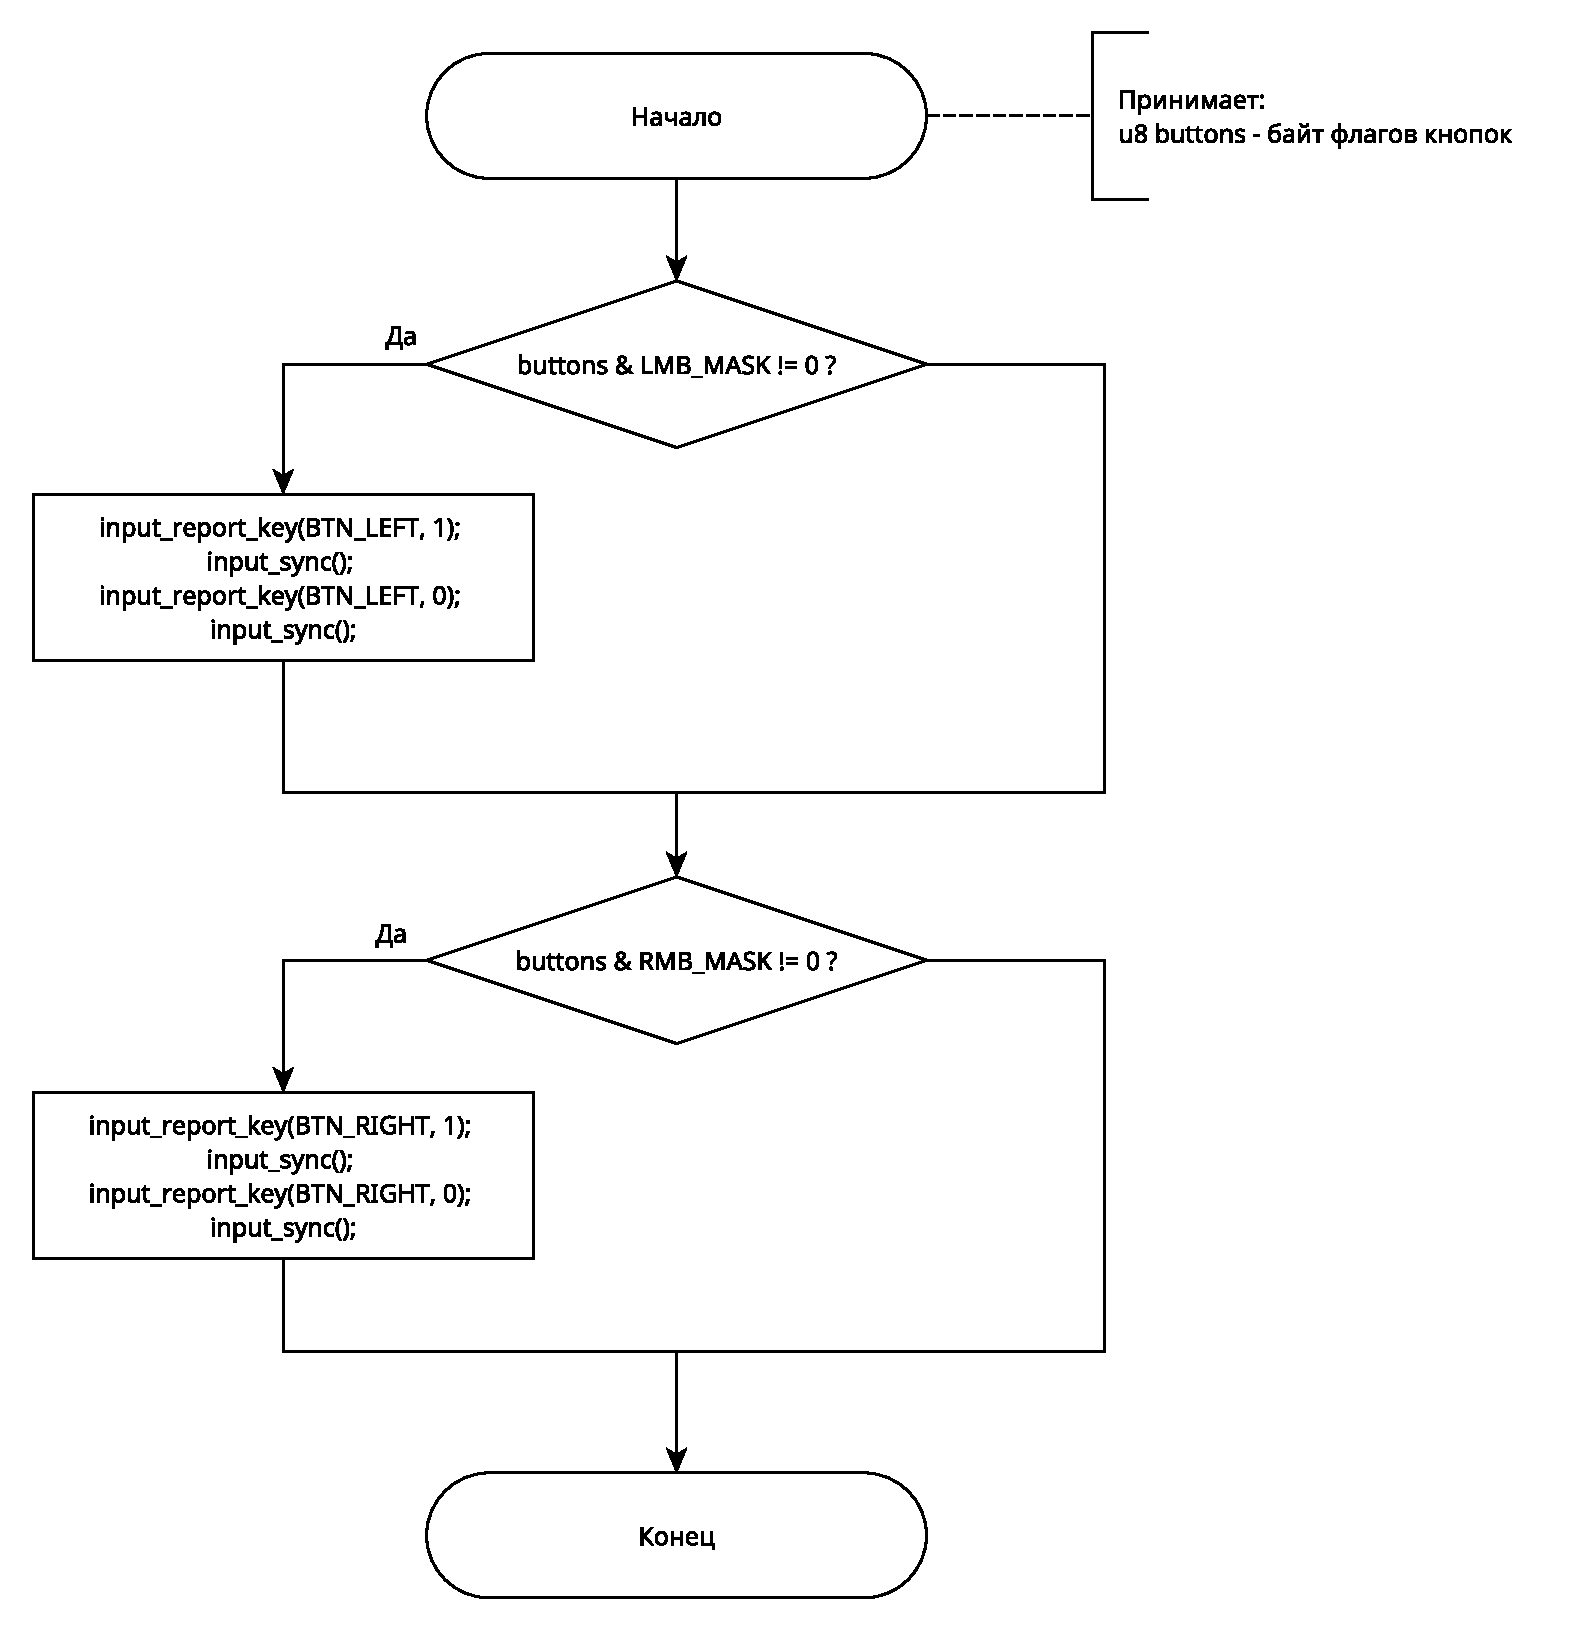
\includegraphics[height=0.7\textheight]{handle_buttons.pdf}
	\caption{Схема алгоритма обработки нажатий кнопок мыши \lstinline|handle_buttons|}
	\label{fig:handle-buttons-scheme}
\end{figure}
\clearpage

Обработка движения курсора реализована в функции \lstinline|handle_movement|. Функция восстанавливает из четырёх байт 16-разрядные смещения по осям, масштабирует их с использованием коэффициента \lstinline|speed_mult| в формате Q16.16 и, в зависимости от значения \lstinline|interp_steps|, либо разбивает движение на несколько мелких шагов с генерацией последовательности событий \lstinline|REL_X| и \lstinline|REL_Y|, либо передаёт смещения единым событием. В обоих случаях каждое изменение сопровождается вызовом \lstinline|input_sync| для фиксации событий подсистемой ввода. Алгоритм функции \lstinline|handle_movement| представлен на рис.~\ref{fig:handle-movement-scheme}.


\begin{figure}[h!]
	\centering
	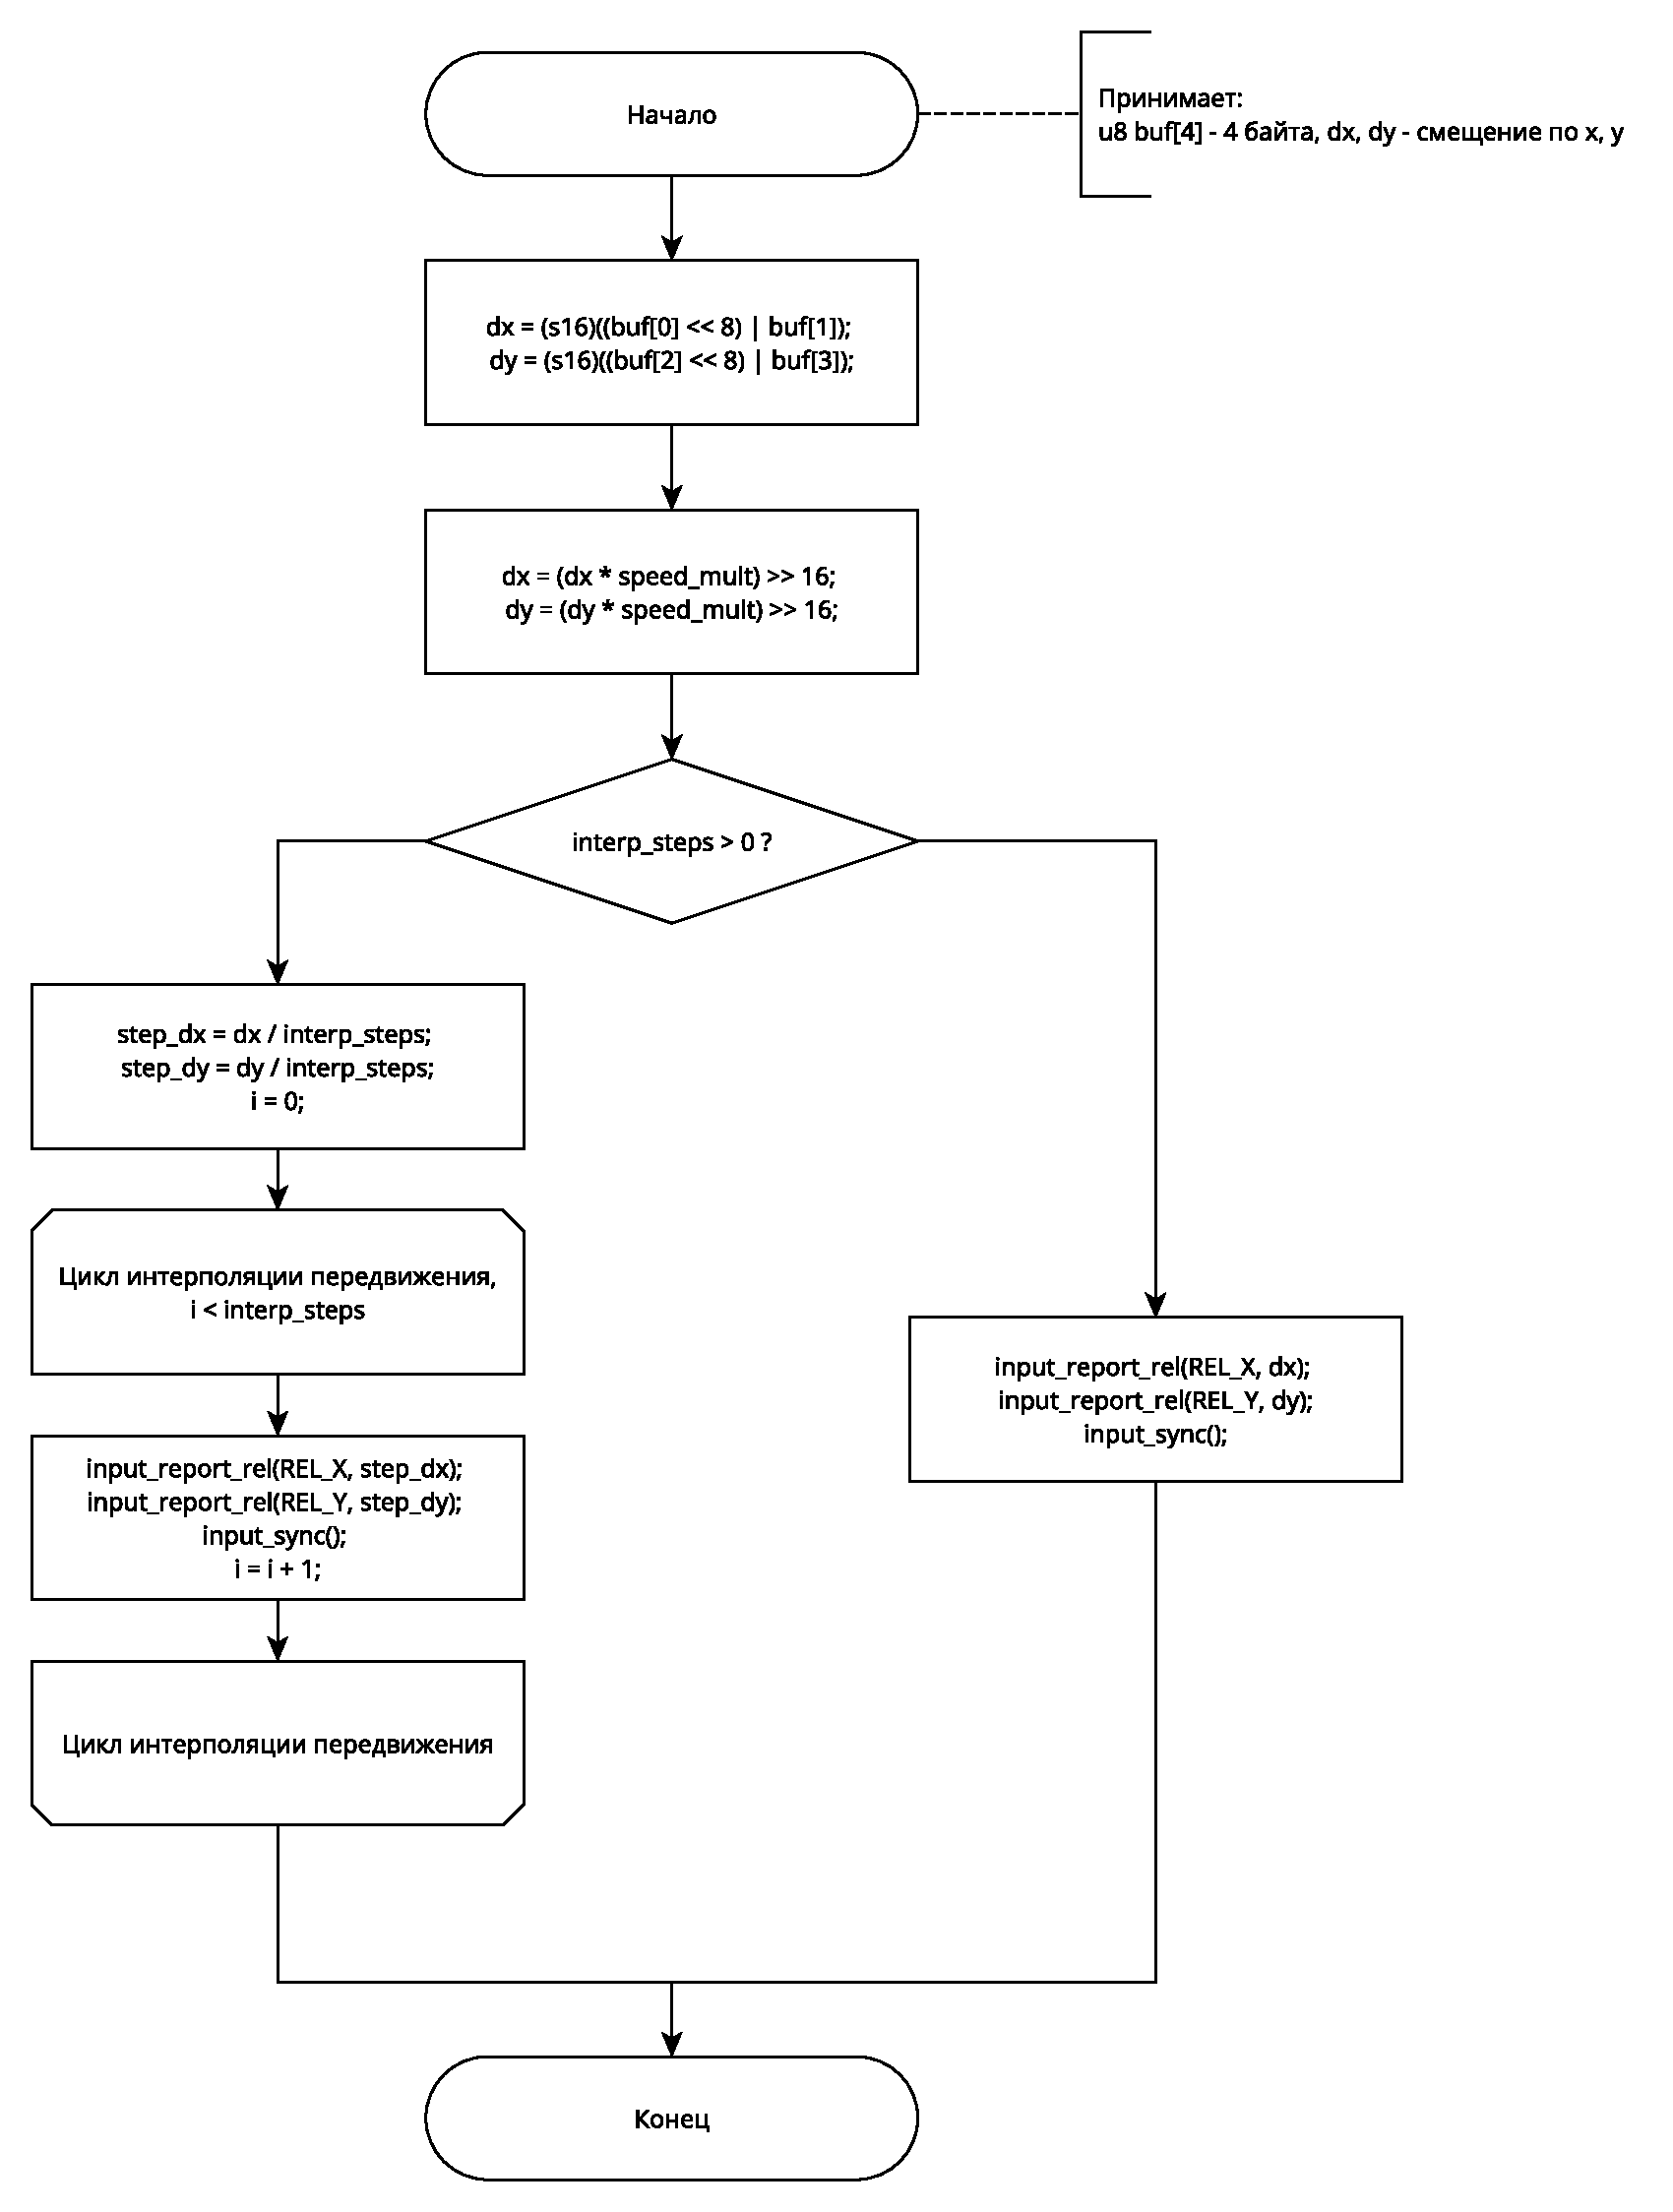
\includegraphics[width=0.7\textwidth]{handle_movement.pdf}
	\caption{Схема алгоритма обработки движения курсора \lstinline|handle_movement|}
	\label{fig:handle-movement-scheme}
\end{figure}
\clearpage

Завершение работы модуля включает остановку служебного потока, закрытие клиентского и серверного RFCOMM-сокетов, снятие виртуального устройства с регистрации и освобождение ресурсов. Последовательность действий функции \lstinline|pm_exit|, зарегистрированной через \lstinline|module_exit|, приведена на рис.~\ref{fig:module-exit-scheme}~\cite{linux-driver-basics,linux-input-docs}.

\begin{figure}[h!]
	\centering
	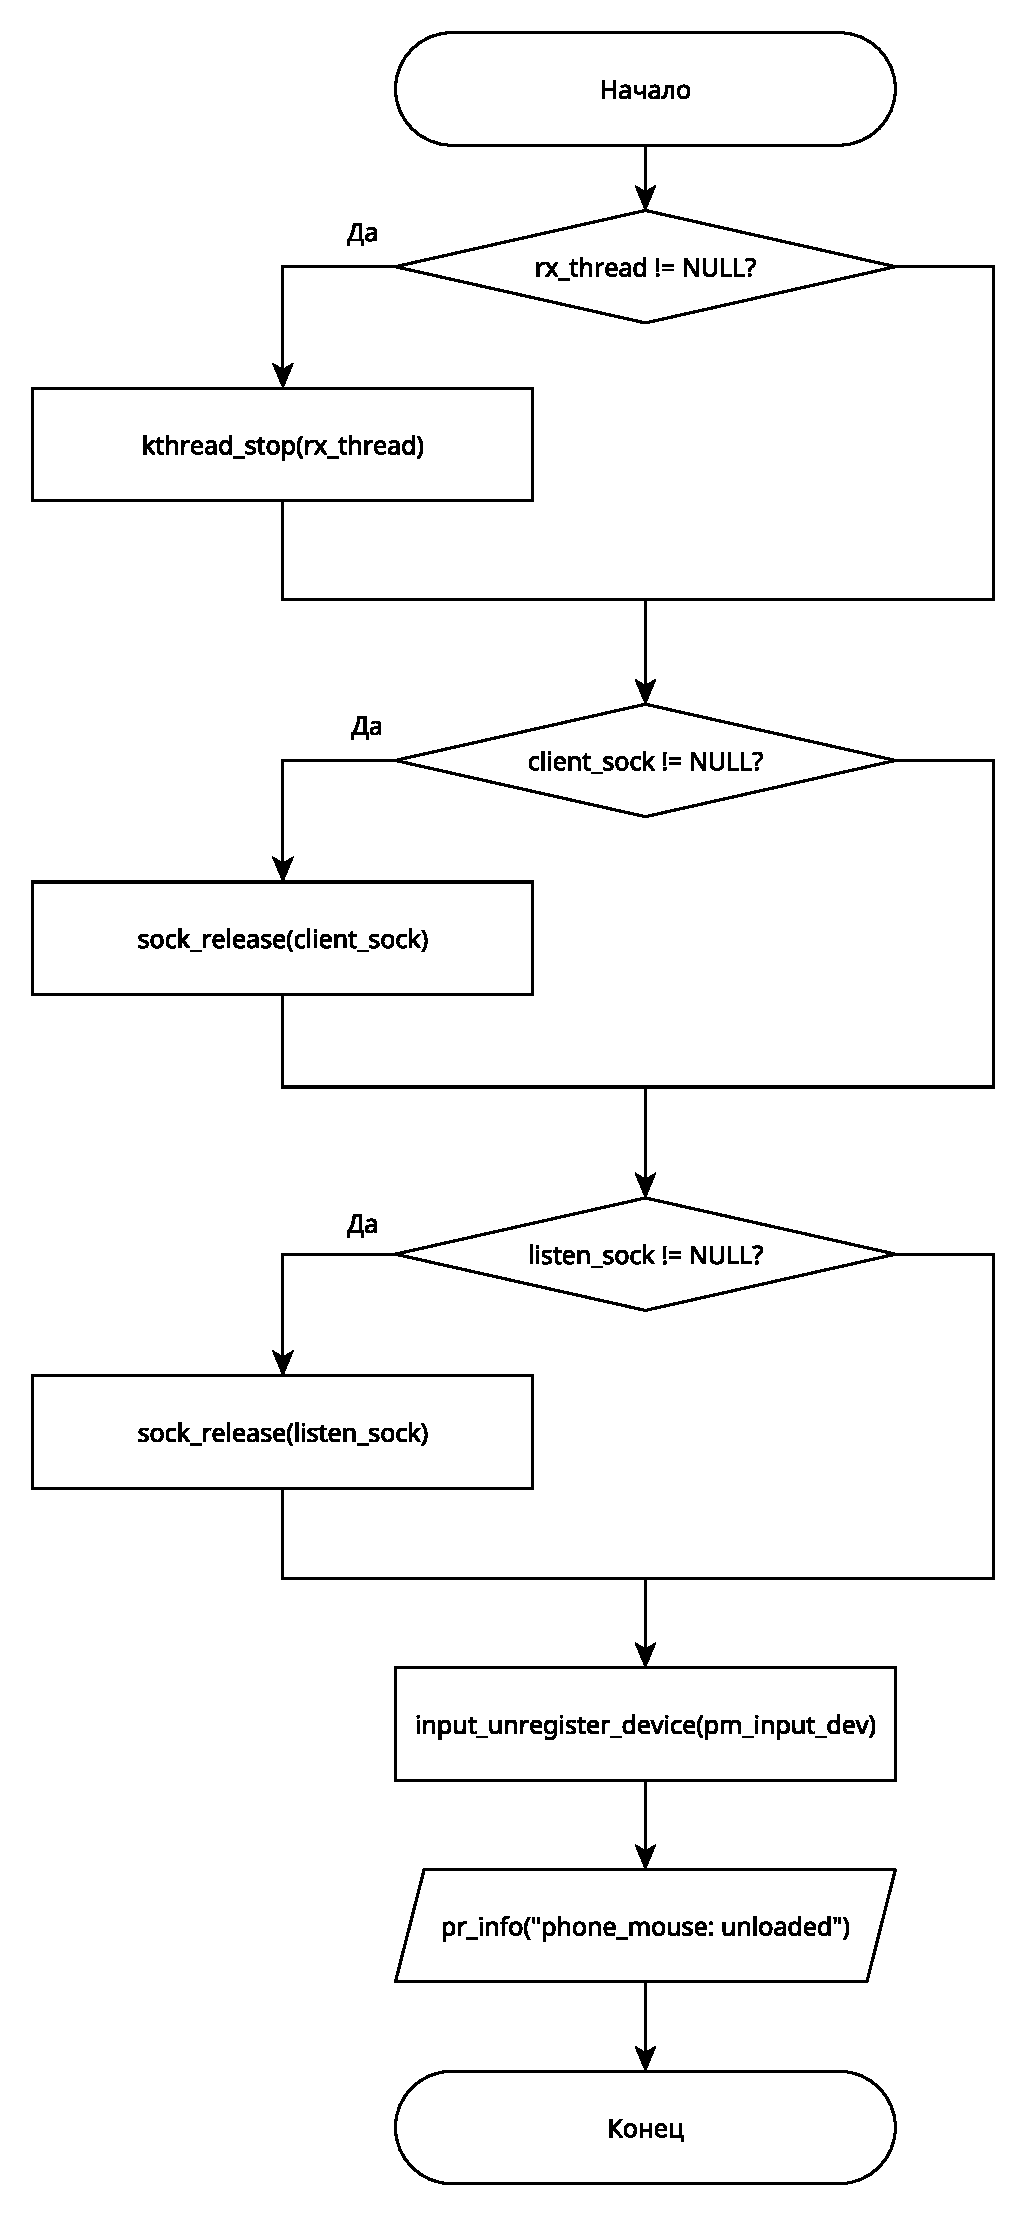
\includegraphics[height=0.7\textheight]{module-exit-scheme.pdf}
	\caption{Схема алгоритма завершения работы модуля ядра \texttt{phone\_mouse\_bt}}
	\label{fig:module-exit-scheme}
\end{figure}
\clearpage

\subsection{Последовательность работы мобильного приложения}

Мобильное приложение реализовано в виде т. н. "Android-активности" (Activity), которая инициализирует пользовательский интерфейс, запускает фоновый поток отправки накопленных смещений курсора, устанавливает Bluetooth-соединение с рабочей станцией и обрабатывает события сенсорного экрана и нажатия кнопок мыши~\cite{android-bt-connect,BluetoothSocket-doc}. Общая последовательность работы основной активности \lstinline|MainActivity| представлена на рис.~\ref{fig:app-main-activity}: при создании активности выполняется настройка интерфейса, запуск фонового потока отправки движения, восстановление сохранённого MAC-адреса, установка обработчиков для поля ввода MAC-адреса, кнопок мыши и области touchpad, а также, при наличии сохранённого адреса, инициируется подключение к рабочей станции.

\begin{figure}[h!]
	\centering
	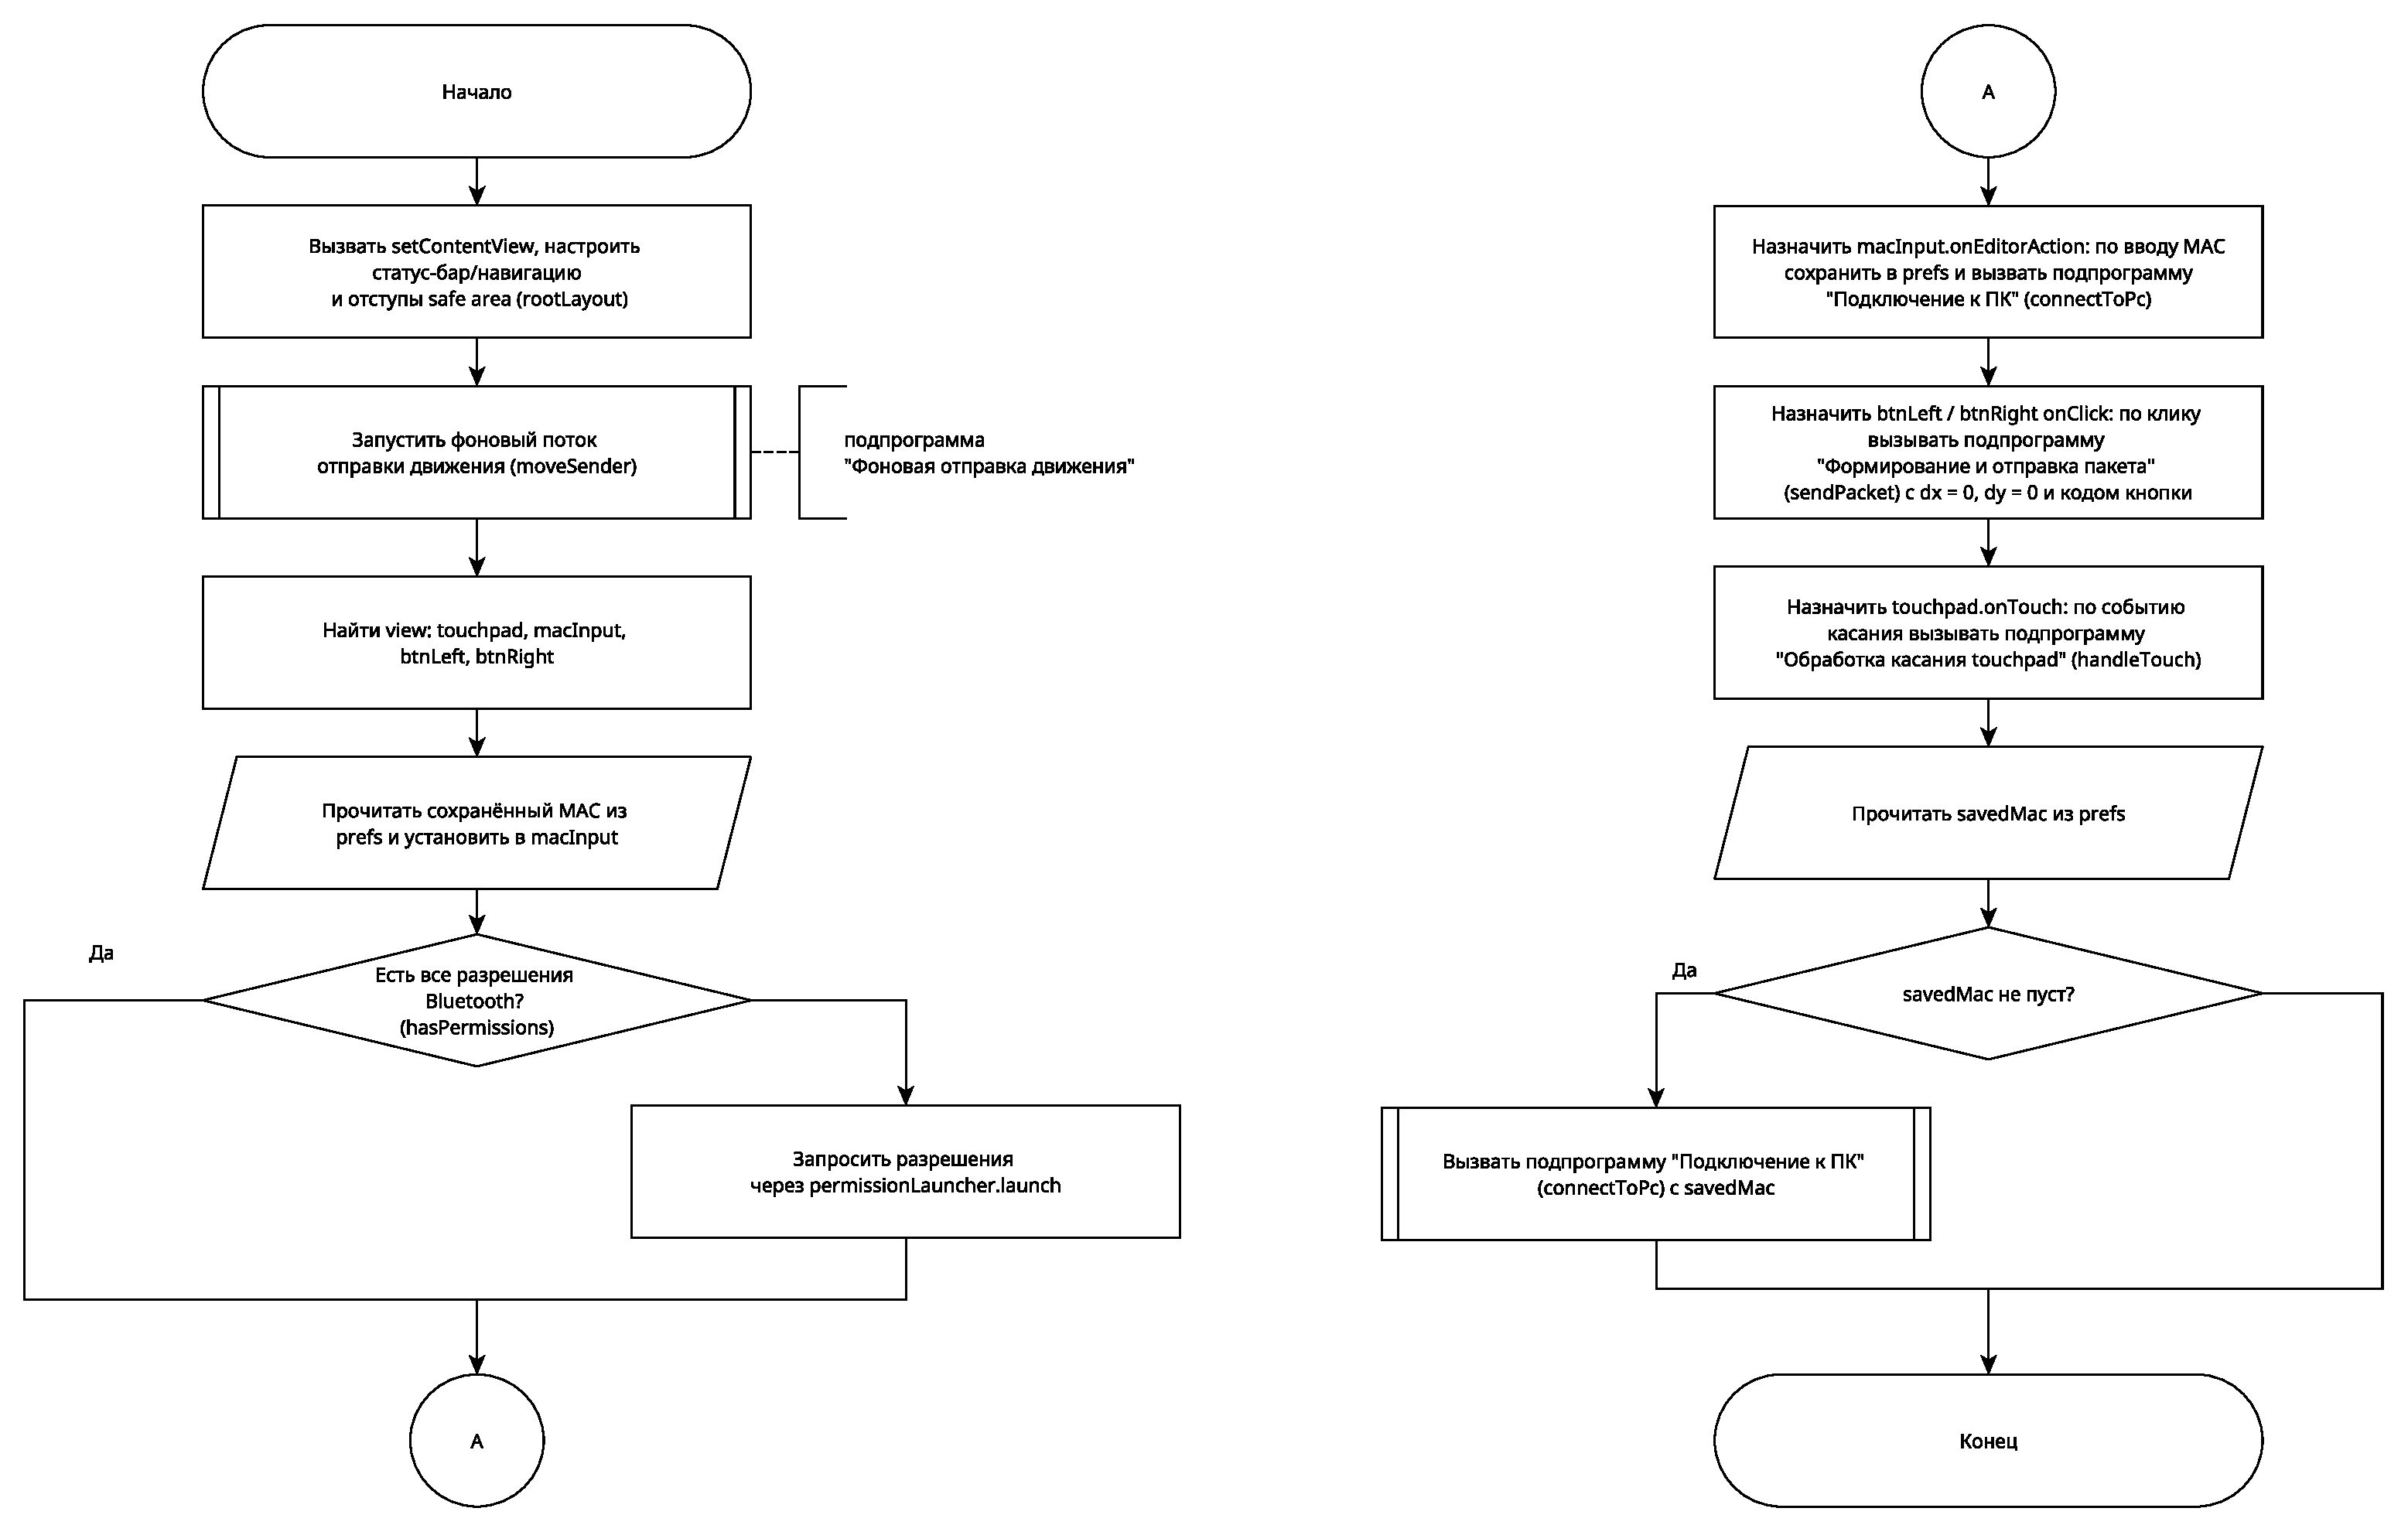
\includegraphics[width=0.9\textwidth]{AppMainActivity.pdf}
	\caption{Схема алгоритма работы основной активности мобильного приложения}
	\label{fig:app-main-activity}
\end{figure}
\clearpage

Отправка накопленных смещений курсора реализована в отдельном потоке, который с фиксированным интервалом времени считывает значения переменных \lstinline|pendingDx| и \lstinline|pendingDy|, обнуляет накопленные значения и, при ненулевых смещениях, формирует пакет данных о смещении курсора, которая отправляется на устройство-обработчик с помощью вызова \lstinline|sendPacket|. Алгоритм работы данного потока показан на рис.~\ref{fig:sendpacket-thread}.

\begin{figure}[h!]
	\centering
	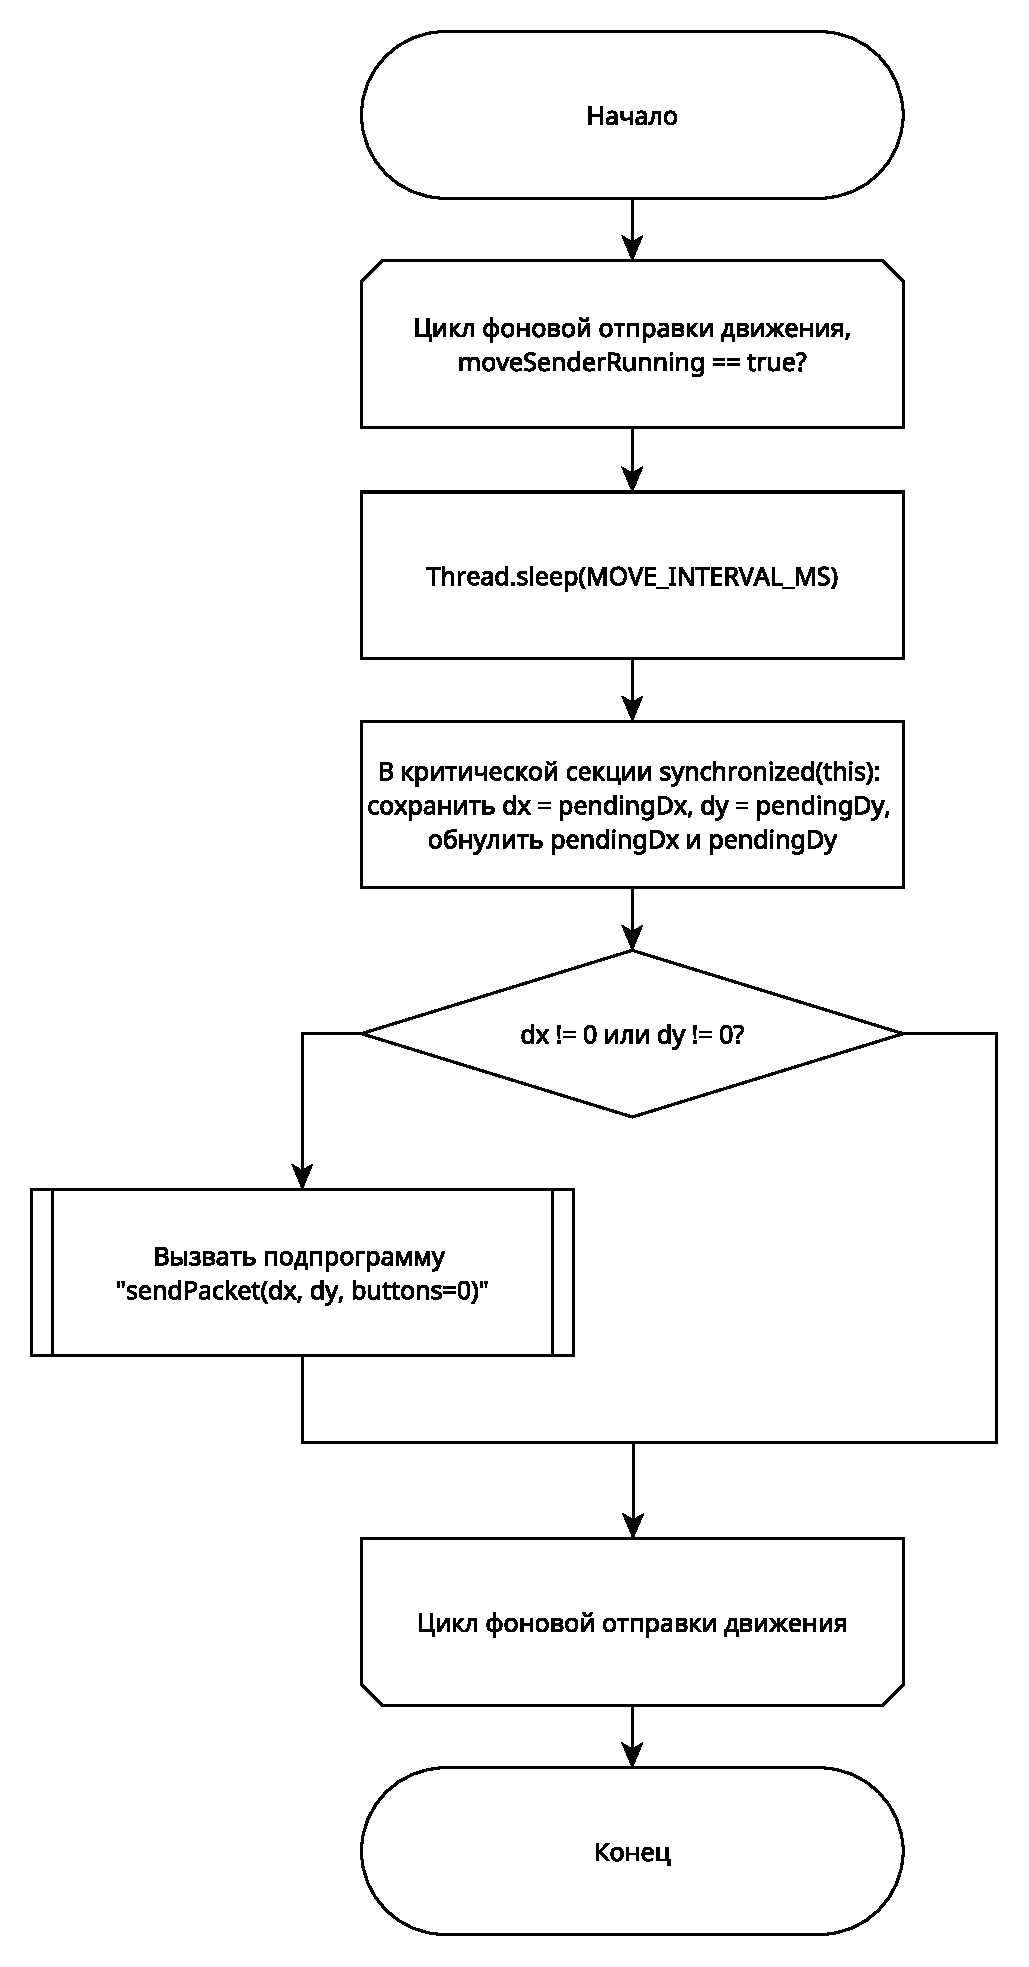
\includegraphics[height=0.7\textheight]{SendPacketThread.pdf}
	\caption{Схема алгоритма фонового потока отправки накопленных смещений}
	\label{fig:sendpacket-thread}
\end{figure}
\clearpage

Функция \lstinline|sendPacket| формирует бинарное сообщения протокола из смещений по осям и битовой маски кнопок мыши, проверяет наличие открытого выходного потока, упаковывает значения в массив из пяти байт и выполняет запись массива в \lstinline|OutputStream|, игнорируя исключения ввода-вывода. Последовательность действий функции \lstinline|sendPacket| представлена на рис.~\ref{fig:sendpacket-func}.

\begin{figure}[h!]
	\centering
	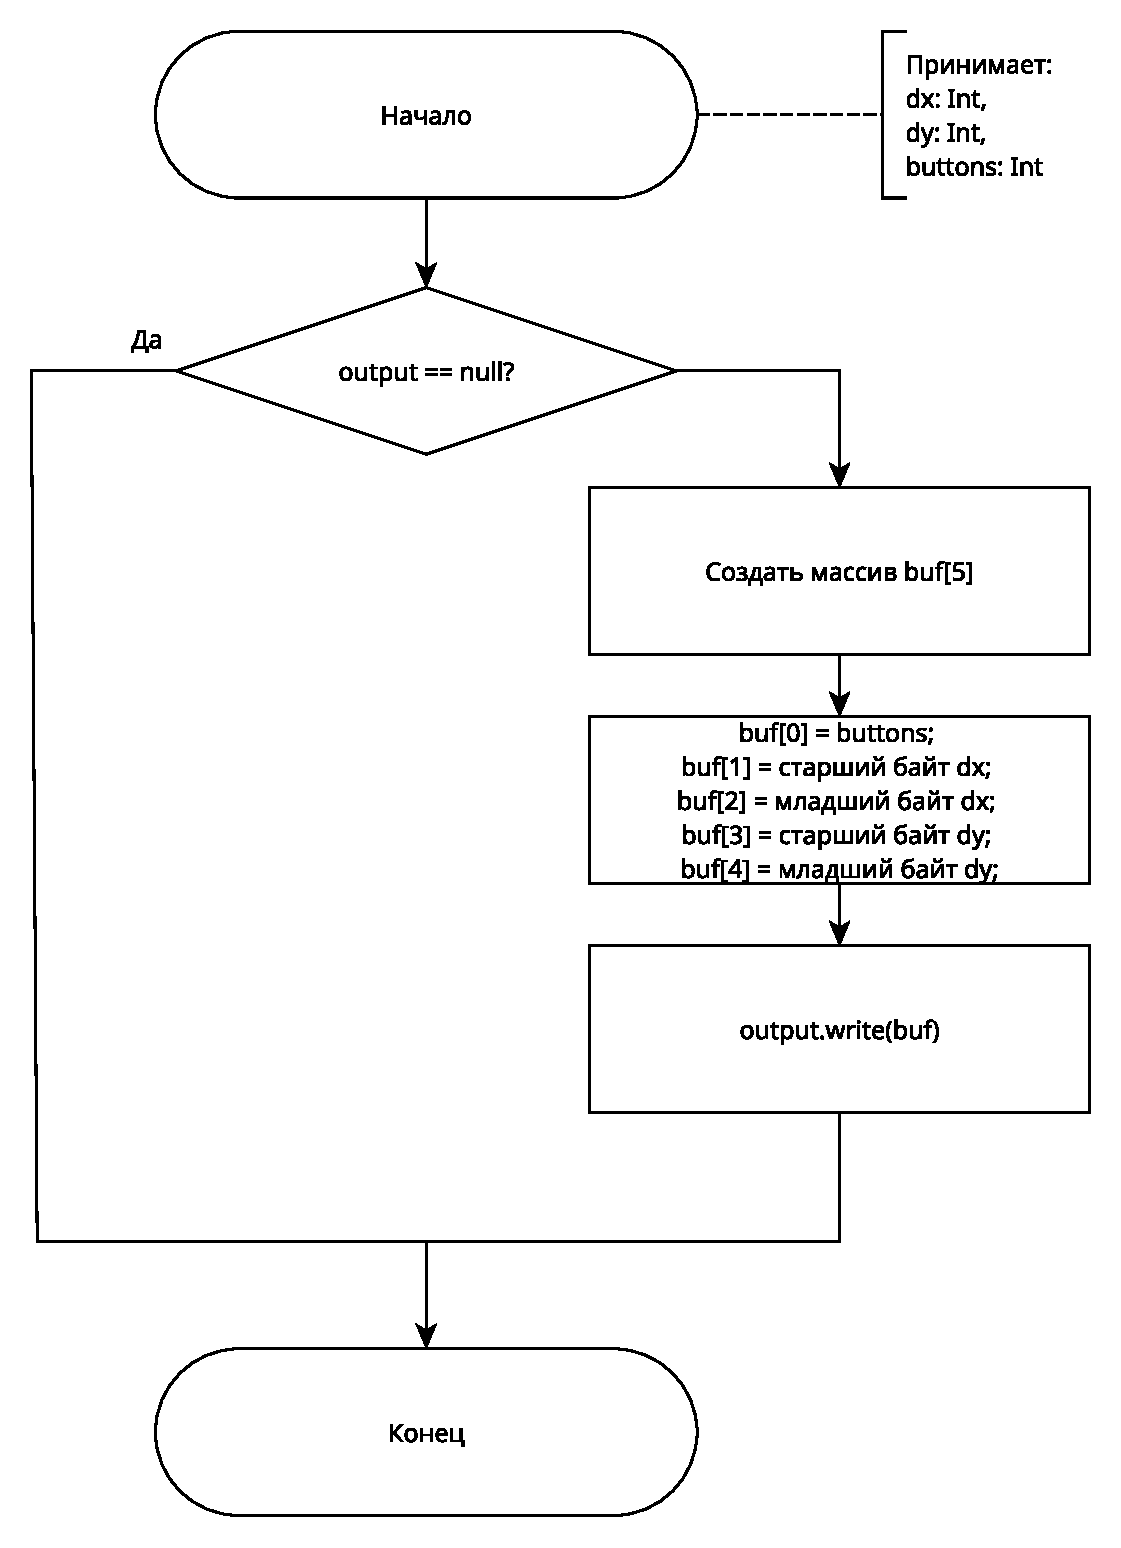
\includegraphics[width=0.8\textwidth]{SendPacket.pdf}
	\caption{Схема алгоритма формирования и отправки пакета команд \lstinline|sendPacket|}
	\label{fig:sendpacket-func}
\end{figure}
\clearpage

Установление соединения с целевым устройством выполняется функцией \lstinline|connectToPc|, которая проверяет корректность введённого MAC-адреса, получает адаптер Bluetooth, инициирует фоновый поток подключения, создаёт RFCOMM-сокет к указанному каналу, выполняет соединение и сохраняет \lstinline|BluetoothSocket| и поток вывода. В случае успеха и при ошибках пользователю отображаются диагностические сообщения. Общий алгоритм функции \lstinline|connectToPc| показан на рис.~\ref{fig:connect-to-pc}, а внутренний поток подключения, использующий вызовы сокета и обработку исключений, представлен отдельно на рис.~\ref{fig:connect-to-pc-thread}.

\begin{figure}[h!]
	\centering
	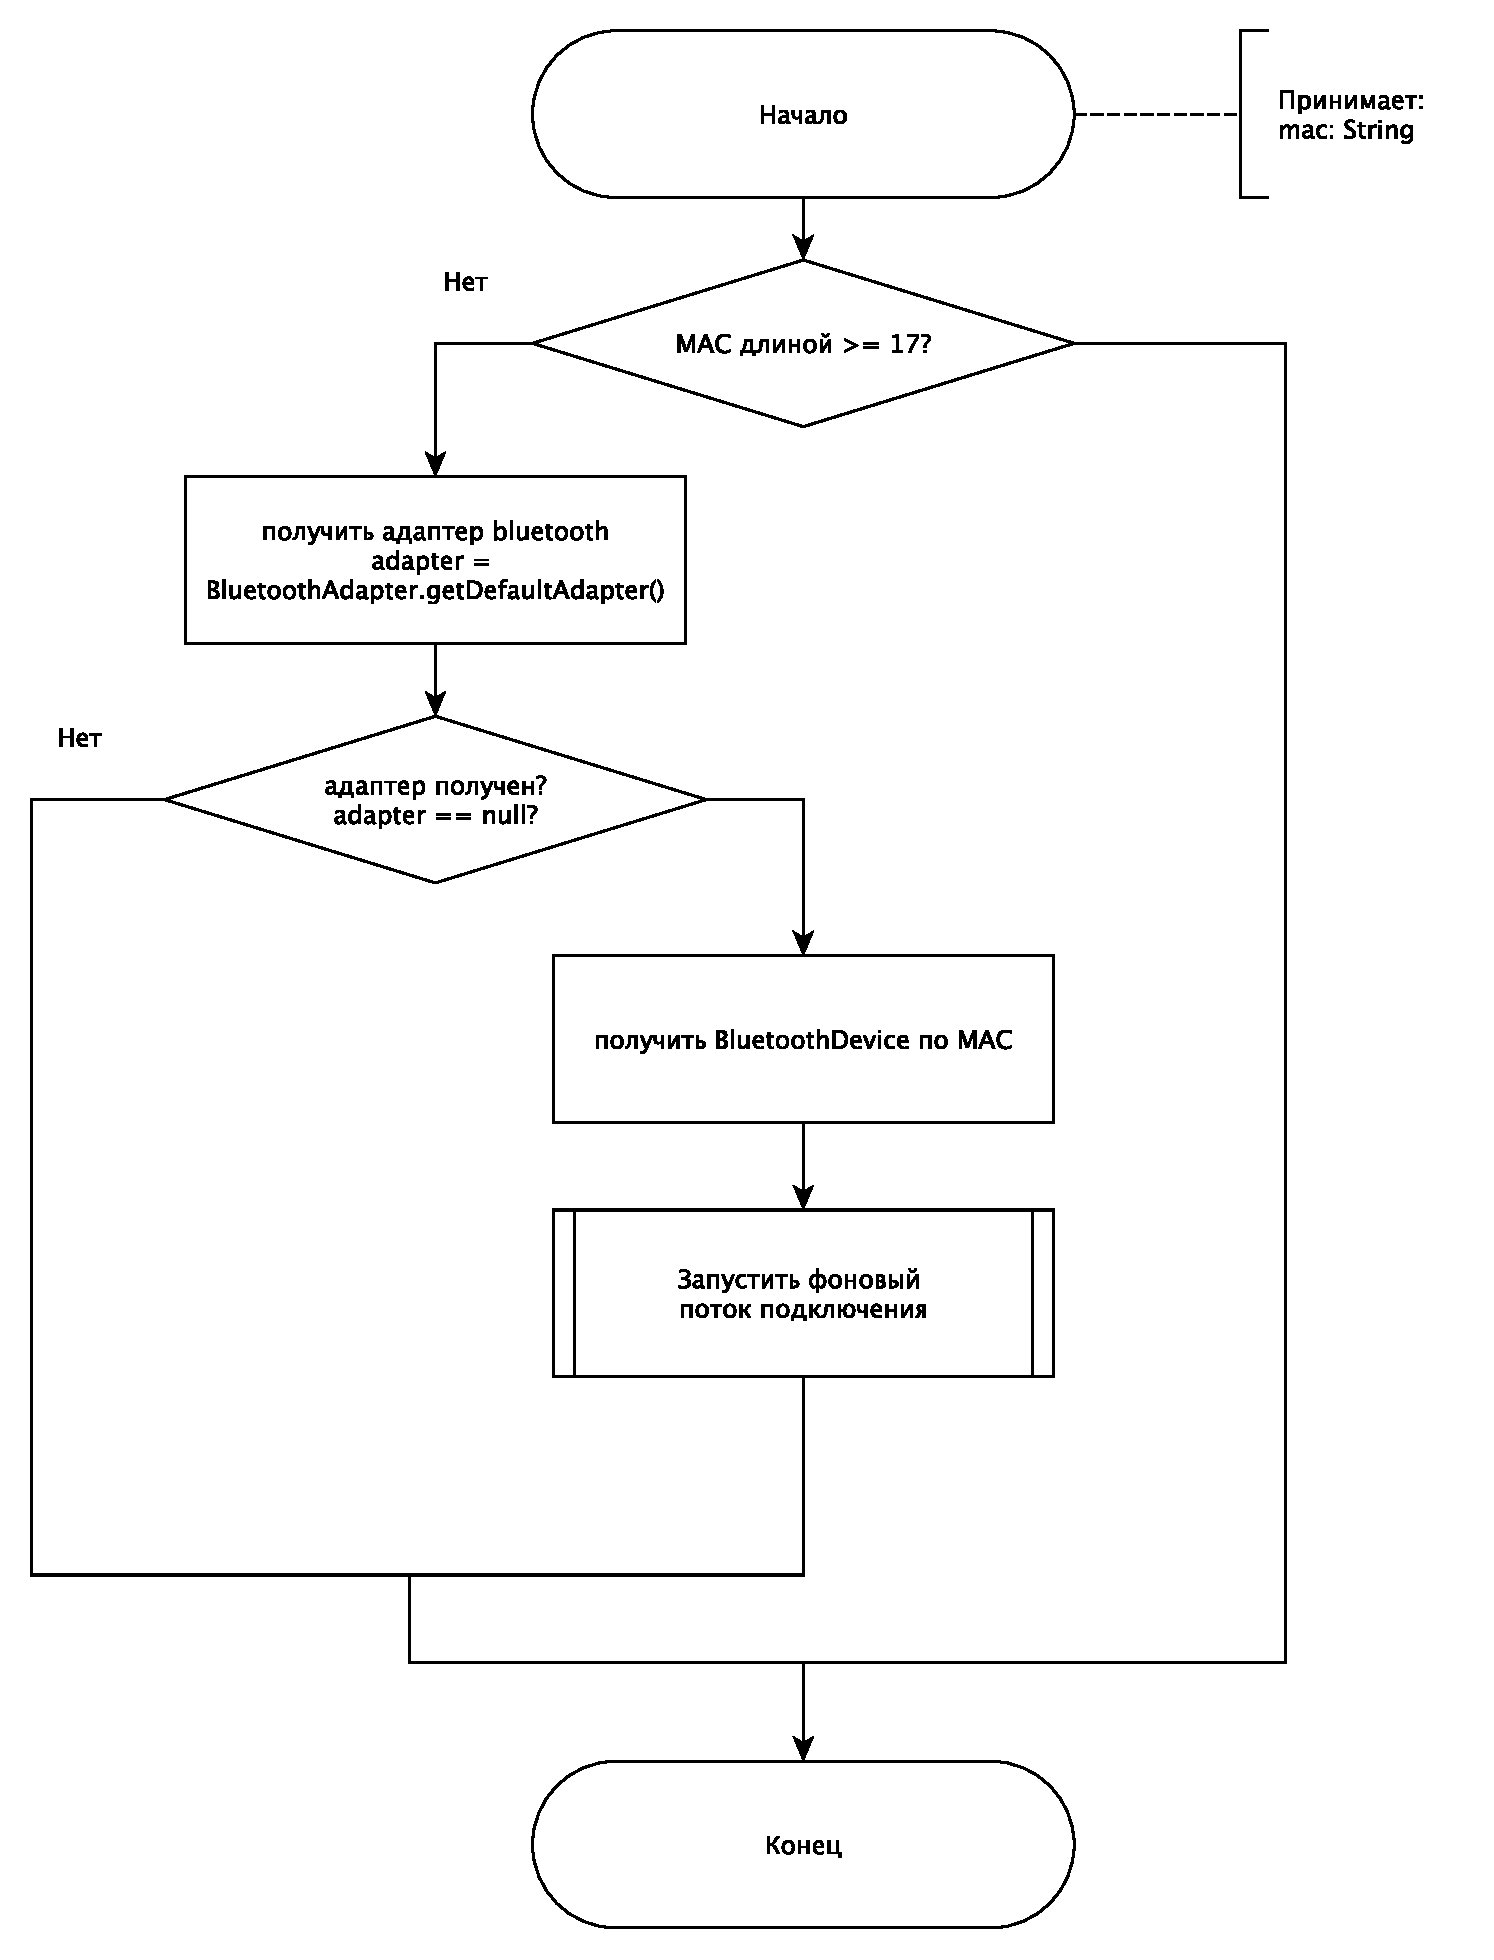
\includegraphics[height=0.7\textheight]{ConnectToPc.pdf}
	\caption{Схема алгоритма функции подключения к рабочей станции \lstinline|connectToPc|}
	\label{fig:connect-to-pc}
\end{figure}
\clearpage

\begin{figure}[h!]
	\centering
	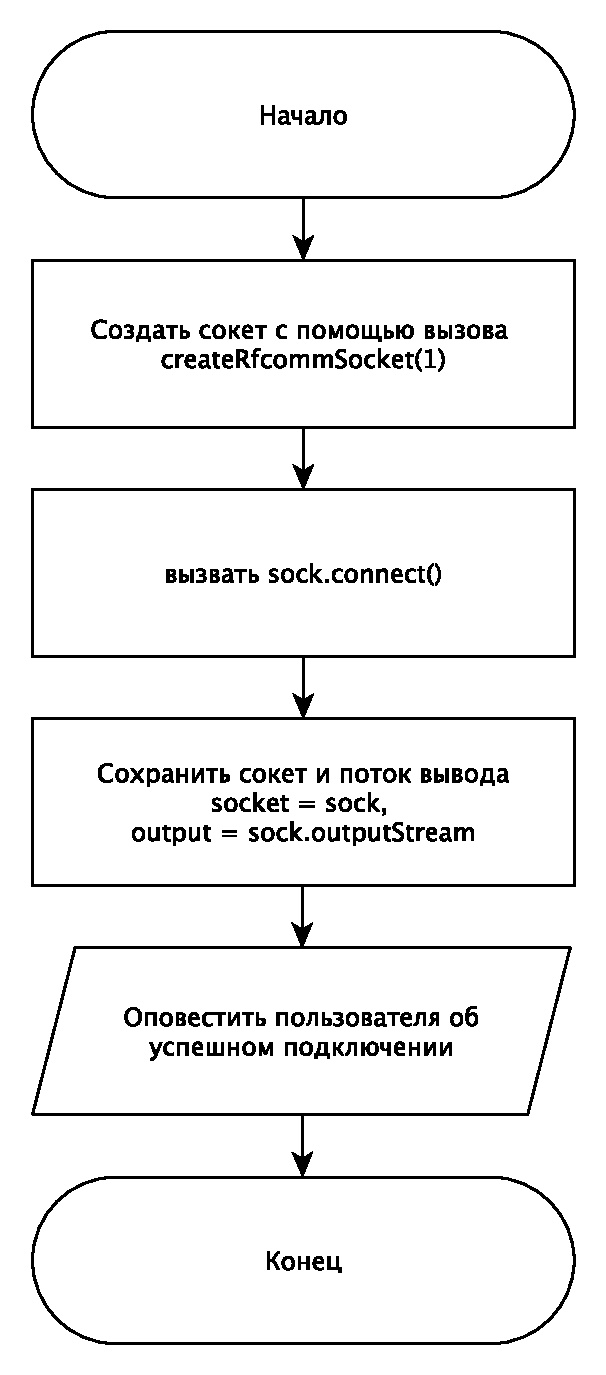
\includegraphics[height=0.9\textheight]{ConnectToPcInnerThread.pdf}
	\caption{Схема алгоритма внутреннего потока установления RFCOMM-соединения}
	\label{fig:connect-to-pc-thread}
\end{figure}
\clearpage


Обработка движения пальца по сенсорной области реализована в функции \lstinline|handleTouch|, которая по событию \lstinline|ACTION_DOWN| запоминает исходные координаты и сбрасывает флаг первого движения, а по событиям \lstinline|ACTION_MOVE| вычисляет относительные смещения по осям, обновляет координаты последнего касания и в критической секции увеличивает накопленные значения \lstinline|pendingDx| и \lstinline|pendingDy|. Эта логика отражена на рис.~\ref{fig:handle-touch}. Накопленные таким образом смещения затем периодически считываются фоновым потоком, изображённым на рис.~\ref{fig:sendpacket-thread}, и передаются в драйвер.

\begin{figure}[h!]
	\centering
	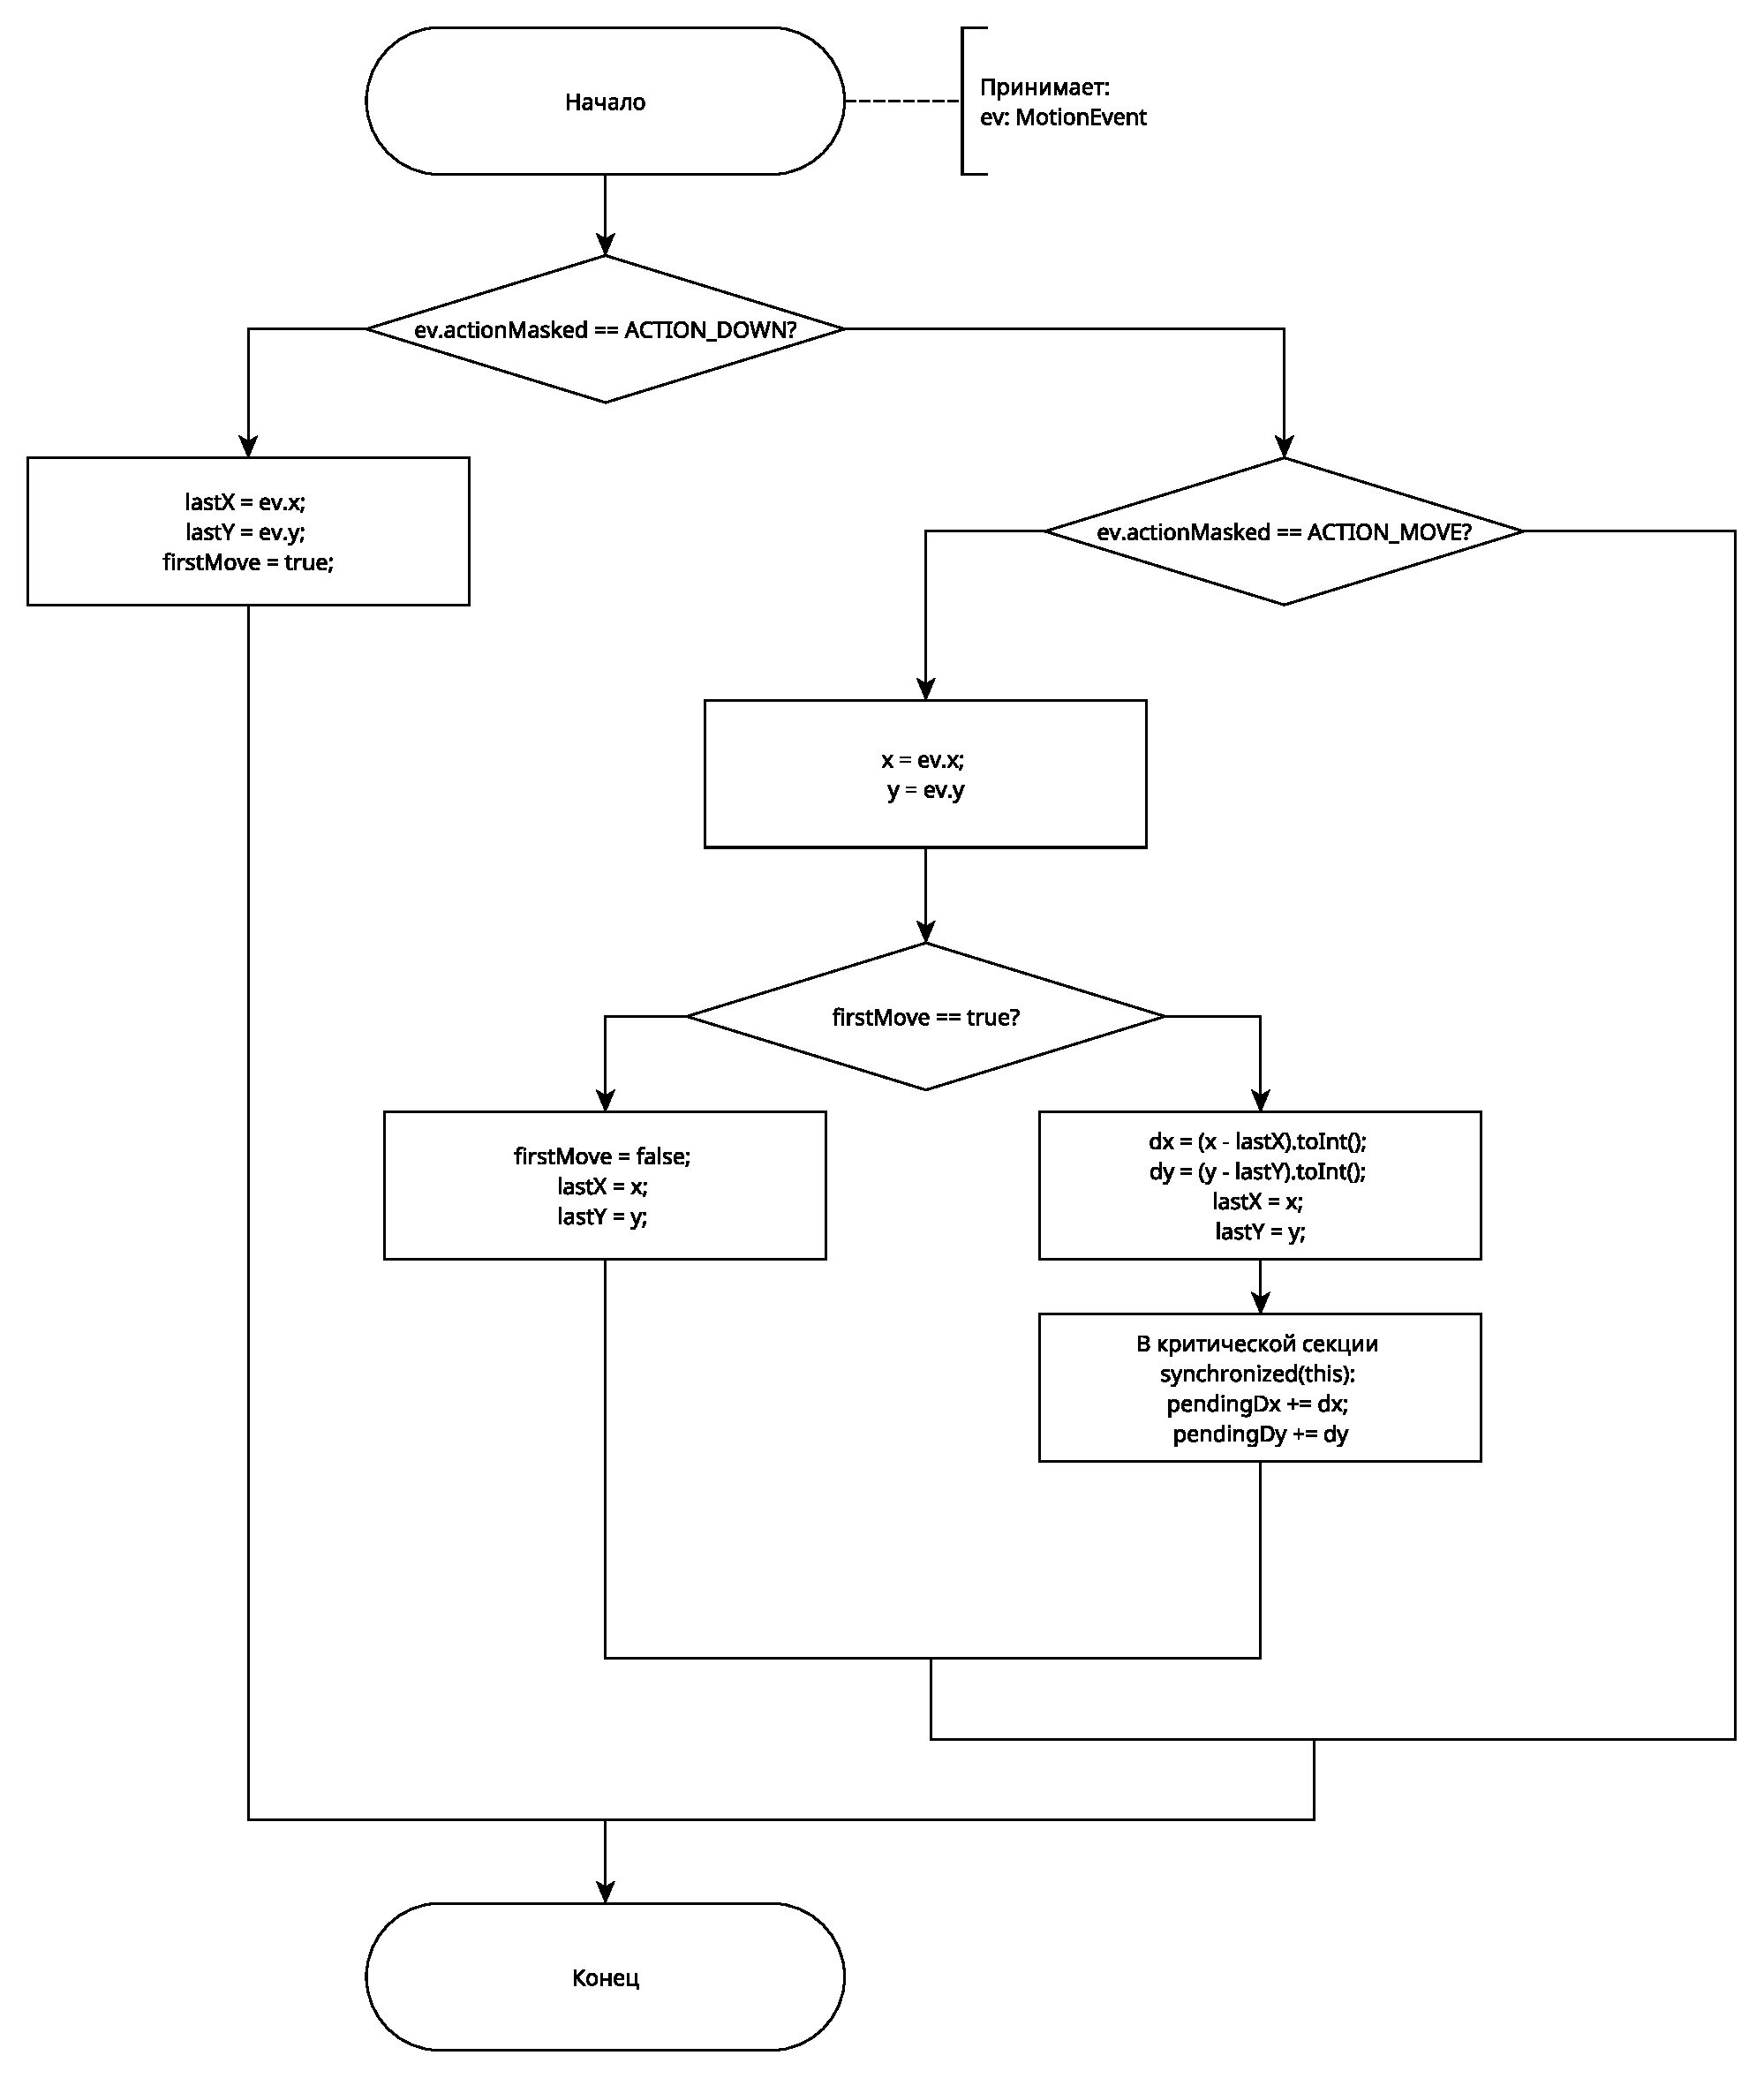
\includegraphics[width=0.9\textwidth]{HandleTouch.pdf}
	\caption{Схема алгоритма обработки касаний на области touchpad \lstinline|handleTouch|}
	\label{fig:handle-touch}
\end{figure}
\clearpage


\section{Технологический раздел}

\subsection{Выбор языка и среды программирования}

Загружаемый модуль ядра реализован на языке программирования C. 
Ядро Linux и большинство драйверов и загружаемых модулей традиционно реализуются на C, а интерфейсы ядровых API, включая подсистему ввода, работу с сокетами и потоками, определяются в терминах C-структур и функций~\cite{c-lang-docs,linux-driver-basics,linux-input-docs}. 
Язык C предоставляет контроль над управлением памятью, представлением структур данных и взаимодействием с заголовочными файлами ядра, а также поддерживается стандартным инструментарием сборки модулей ядра на основе подсистемы Kbuild~\cite{linux-driver-basics}.
Таким образом, язык программирования C является достаточным для реализации драйвера.

Сборка модуля ядра выполняется с использованием стандартной инфраструктуры сборки ядра Linux и утилиты \texttt{make}. Для интеграции с подсистемой Kbuild используется конфигурационный файл \texttt{Makefile}, в котором описаны цели сборки, имя модуля и перечень исходных файлов~\cite{linux-driver-basics}.

Мобильное приложение разработано на языке Kotlin.
Этот язык официально поддерживается в экосистеме Android и интегрирован с Android Studio и системой сборки Gradle, что обеспечивает доступ к Android SDK и библиотекам платформы, включая API Bluetooth~\cite{kotlin-site,android-bt-connect}. 
Совместимость с Java-API позволяет использовать классы \lstinline|BluetoothAdapter|, \lstinline|BluetoothDevice| и \lstinline|BluetoothSocket| непосредственно из Kotlin-кода~\cite{android-bt-connect,BluetoothSocket-doc}.
Таким образом, Kotlin обладает достаточными возможностями для реализации клиентского приложения, а также поддержания связи с модулем ядра на целевом устройстве.

% Выбор C для модуля ядра и Kotlin для мобильного приложения обеспечивает использование низкоуровневых интерфейсов ядра Linux на стороне драйвера и высокоуровневого SDK на стороне Android-приложения, что соответствует постановке задачи по разработке загружаемого модуля и сопряжённого клиента~\cite{linux-driver-basics,android-bt-connect}.

\subsection{Реализация загружаемого модуля ядра Linux}

\subsubsection*{Структуры данных и состояние драйвера}

Загружаемый модуль ядра хранит состояние виртуального устройства мыши и параметры протокола обмена в собственных структурах данных. Основой для интеграции с подсистемой ввода является структура \lstinline|struct input_dev| (представлена в листинге~\ref{lst:input_dev}), которая содержит идентификаторы устройства, указатели на функции обратного вызова и описания поддерживаемых типов и кодов событий~\cite{linux-input-docs,input-programming}. Дополнительно используются структуры для хранения текущих состояний кнопок и параметров RFCOMM-соединения.
Фрагмент объявления структур данных драйвера приведён в листинге~\ref{lst:definitions}.

\begin{lstlisting}[language=C,caption={Структура \texttt{input\_dev}},label={lst:input_dev}]
	struct input_dev {
		const char * name;
		const char * phys;
		const char * uniq;
		struct input_id id;
		unsigned long propbit;
		unsigned long evbit;
		unsigned long keybit;
		unsigned long relbit;
		unsigned long absbit;
		unsigned long mscbit;
		unsigned long ledbit;
		unsigned long sndbit;
		unsigned long ffbit;
		unsigned long swbit;
		unsigned int hint_events_per_packet;
		unsigned int keycodemax;
		unsigned int keycodesize;
		void * keycode;
		int (* setkeycode) (struct input_dev *dev,const struct input_keymap_entry *ke, unsigned int *old_keycode);
		int (* getkeycode) (struct input_dev *dev, struct input_keymap_entry *ke);
		struct ff_device * ff;
		unsigned int repeat_key;
		struct timer_list timer;
		int rep;
		struct input_mt * mt;
		struct input_absinfo * absinfo;
		unsigned long key;
		unsigned long led;
		unsigned long snd;
		unsigned long sw;
		int (* open) (struct input_dev *dev);
		void (* close) (struct input_dev *dev);
		int (* flush) (struct input_dev *dev, struct file *file);
		int (* event) (struct input_dev *dev, unsigned int type, unsigned int code, int value);
		struct input_handle __rcu * grab;
		spinlock_t event_lock;
		struct mutex mutex;
		unsigned int users;
		bool going_away;
		struct device dev;
		struct list_head h_list;
		struct list_head node;
		unsigned int num_vals;
		unsigned int max_vals;
		struct input_value * vals;
		bool devres_managed;
	};
\end{lstlisting}

\begin{lstlisting}[language=C,caption={Фрагмент объявления структур данных драйвера \texttt{phone\_mouse\_bt}},label={lst:definitions}]
	/* Виртуальное устройство мыши в подсистеме input */
	static struct input_dev *pm_input_dev;
	
	/* RFCOMM-сокеты для ожидания и обслуживания соединения */
	static struct socket *listen_sock;
	static struct socket *client_sock;
	
	/* Служебный поток приёма пакетов от телефона */
	static struct task_struct *rx_thread;
	
	/* Параметры обработки движения */
	static int interp_steps = 0;   /* число шагов интерполяции движения */
	static int speed_mult;         /* коэффициент скорости в формате Q16.16 */
	
	/* Маски кнопок в протокольном байте buttons */
	#define LMB_MASK 0x01
	#define RMB_MASK 0x02
\end{lstlisting}

\subsubsection*{Точки входа модуля и функции обработки}

Точки входа загружаемого модуля определяются функциями инициализации и завершения, регистрируемыми макросами \lstinline|module_init| и \lstinline|module_exit|~\cite{linux-driver-basics}. В функции инициализации выполняются:
\begin{itemize}
	\item создание и настройка объекта \lstinline|struct input_dev| и регистрация виртуального устройства мыши в подсистеме ввода;
	\item инициализация структур данных состояния драйвера;
	\item создание серверного RFCOMM-сокета и его привязка к выбранному каналу;
	\item запуск служебного потока ядра с помощью \lstinline|kthread_run| для обработки соединения и входящих команд~\cite{linux-kthread-man,linux-rfcomm-core}.
\end{itemize}

Функция завершения выполняет остановку служебного потока, закрытие RFCOMM-сокета, снятие виртуального устройства с регистрации и освобождение всех выделенных ресурсов~\cite{linux-driver-basics}.

Функции инициализации и завершения драйвера модуля приведены в листингах~\ref{lst:init}~и~\ref{lst:exit} соответственно.

\begin{lstlisting}[language=C,caption={Функция инициализации модуля},label={lst:init}]
	static int __init pm_init(void) {
		int err;
		struct sockaddr_rc addr = {0};
		
		if (interp_steps < 0) {
			pr_err("phone_mouse_bt: ERROR: interp_steps must be >= 0 (got %d)\n",
			interp_steps);
			return -EINVAL;
		}
		
		speed_mult = (speed_pct * 65536) / 100;
		pr_info("phone_mouse_bt: speed coefficient = %d (Q16.16)\n", speed_mult);
		
		// Allocate new input device
		pm_input_dev = input_allocate_device();
		if (!pm_input_dev)
		return -ENOMEM;
		
		pm_input_dev->name = "Bluetooth Phone Mouse";
		pm_input_dev->id.bustype = BUS_BLUETOOTH;
		
		__set_bit(EV_KEY, pm_input_dev->evbit);
		__set_bit(EV_REL, pm_input_dev->evbit);
		
		__set_bit(BTN_LEFT, pm_input_dev->keybit);
		__set_bit(BTN_RIGHT, pm_input_dev->keybit);
		
		__set_bit(REL_X, pm_input_dev->relbit);
		__set_bit(REL_Y, pm_input_dev->relbit);
		
		err = input_register_device(pm_input_dev);
		if (err)
		return err;
		
		// RFCOMM socket
		err = sock_create_kern(&init_net, PF_BLUETOOTH, SOCK_STREAM, BTPROTO_RFCOMM,
		&listen_sock);
		if (err < 0) {
			pr_err("phone_mouse: sock_create_kern failed\n");
			return err;
		}
		
		addr.rc_family = AF_BLUETOOTH;
		bacpy(&addr.rc_bdaddr, BDADDR_ANY);
		addr.rc_channel = bt_listen_channel;
		
		err = listen_sock->ops->bind(listen_sock, (struct sockaddr *)&addr,
		sizeof(addr));
		if (err < 0) {
			pr_err("phone_mouse: bind failed\n");
			return err;
		}
		
		err = listen_sock->ops->listen(listen_sock, 1);
		if (err < 0) {
			pr_err("phone_mouse: listen failed\n");
			return err;
		}
		
		// Main loop in kernel thread
		rx_thread = kthread_run(rx_loop, NULL, "phone_mouse_rx");
		if (IS_ERR(rx_thread)) {
			pr_err("phone_mouse: failed to start thread\n");
			return PTR_ERR(rx_thread);
		}
		
		pr_info("phone_mouse: module loaded, listening RFCOMM channel %d\n",
		bt_listen_channel);
		
		return 0;
	}
\end{lstlisting}

\begin{lstlisting}[language=C,caption={Функция завершения модуля},label={lst:exit}]
	static void __exit pm_exit(void) {
		if (rx_thread)
		kthread_stop(rx_thread);
		
		if (client_sock)
		sock_release(client_sock);
		
		if (listen_sock)
		sock_release(listen_sock);
		
		input_unregister_device(pm_input_dev);
		
		pr_info("phone_mouse: unloaded\n");
	}
\end{lstlisting}

Служебный поток \lstinline|rx_loop| реализует цикл приёма данных из RFCOMM-сокета: при отсутствии активного клиента поток ожидает входящего соединения, после установления соединения периодически читает из сокета фиксированный пакет длиной пять байт, обрабатывает ситуации временного отсутствия данных и разрыва соединения и, для корректных пакетов, передаёт первый байт в функцию \lstinline|handle_buttons|, а четыре следующих байта --- в функцию \lstinline|handle_movement|. Функция \lstinline|handle_buttons| на основе битовой маски кнопок порождает события \lstinline|EV_KEY|, а функция \lstinline|handle_movement| декодирует смещения по осям, масштабирует их и генерирует соответствующие события \lstinline|EV_REL| с последующим вызовом \lstinline|input_sync|~\cite{linux-input-docs,input-programming,bluetooth-core-spec,bluez-rfcomm-wiki}.


\begin{lstlisting}[language=C,caption={Функция служебного потока приёма пакетов по RFCOMM}]
	static int rx_loop(void *data) {
		struct msghdr msg = {0};
		struct kvec vec;
		u8 buf[5];
		
		while (!kthread_should_stop()) {
			
			if (!client_sock) {
				/* Ждём подключения */
				struct socket *new_sock = NULL;
				int r = kernel_accept(listen_sock, &new_sock, 0);
				if (r == 0) {
					client_sock = new_sock;
					pr_info("phone_mouse: client connected!\n");
				} else {
					ssleep(1);
					continue;
				}
			}
			
			vec.iov_base = buf;
			vec.iov_len = sizeof(buf);
			
			int len =
			kernel_recvmsg(client_sock, &msg, &vec, 1, sizeof(buf), MSG_DONTWAIT);
			
			if (len == -EAGAIN) {
				msleep(5);
				continue;
			}
			if (len <= 0) {
				pr_info("phone_mouse: client disconnected\n");
				sock_release(client_sock);
				client_sock = NULL;
				continue;
			}
			if (len < 5)
			continue;
			
			handle_buttons(buf[0]);
			
			handle_movement(&buf[1]);
		}
		
		return 0;
	}
\end{lstlisting}

\begin{lstlisting}[language=C,caption={Функция обработки нажатия кнопки}]
	#define LMB_MASK 0b00000001
	#define RMB_MASK 0b00000010
	static void handle_buttons(u8 buttons) {
		if (buttons & LMB_MASK) {
			input_report_key(pm_input_dev, BTN_LEFT, 1);
			input_sync(pm_input_dev);
			input_report_key(pm_input_dev, BTN_LEFT, 0);
			input_sync(pm_input_dev);
		}
		
		if (buttons & RMB_MASK) {
			input_report_key(pm_input_dev, BTN_RIGHT, 1);
			input_sync(pm_input_dev);
			input_report_key(pm_input_dev, BTN_RIGHT, 0);
			input_sync(pm_input_dev);
		}
	}
\end{lstlisting}

\begin{lstlisting}[language=C,caption={Функция обработки движения курсора}]
	static void handle_movement(u8 buf[4]) {
		s16 dx = (s16)((buf[0] << 8) | buf[1]);
		s16 dy = (s16)((buf[2] << 8) | buf[3]);
		
		dx = (dx * speed_mult) >> 16;
		dy = (dy * speed_mult) >> 16;
		
		if (interp_steps > 0) {
			int step_dx = dx / interp_steps;
			int step_dy = dy / interp_steps;
			
			int i;
			for (i = 0; i < interp_steps; i++) {
				input_report_rel(pm_input_dev, REL_X, step_dx);
				input_report_rel(pm_input_dev, REL_Y, step_dy);
				input_sync(pm_input_dev);
			}
			
			return;
		}
		
		input_report_rel(pm_input_dev, REL_X, dx);
		input_report_rel(pm_input_dev, REL_Y, dy);
		
		input_sync(pm_input_dev);
	}
\end{lstlisting}

\subsubsection*{Сборка модуля ядра}

Сборка модуля ядра выполняется внешней по отношению к дереву исходных текстов ядра командой \texttt{make} с использованием файла \texttt{Makefile}, описывающего цель сборки и исходные файлы. В \texttt{Makefile} используются переменные и правила Kbuild, что позволяет компилировать модуль в соответствии с конфигурацией ядра и подключать необходимые заголовочные файлы~\cite{linux-driver-basics}.

\begin{lstlisting}[language=make,caption={Фрагмент файла Makefile для сборки модуля ядра}]
	obj-m += phone_mouse_bt.o

	KDIR := /lib/modules/$(shell uname -r)/build
	
	PWD  := $(shell pwd)
	
	all:
	$(MAKE) -C $(KDIR) M=$(PWD) modules
	
	clean:
	$(MAKE) -C $(KDIR) M=$(PWD) clean
	
\end{lstlisting}

\subsection{Реализация мобильного приложения для Android}

\subsubsection*{Основные компоненты приложения}

Мобильное приложение реализовано в виде Android-приложения с основной активностью, отвечающей за инициализацию пользовательского интерфейса, установление Bluetooth-соединения и обработку входных событий. Логика обработки касаний и генерации команд размещается в коде активности и связанных с ней обработчиков событий, а обмен данными по Bluetooth --- в отдельном компоненте, использующем объект \lstinline|BluetoothSocket|~\cite{android-bt-connect,BluetoothSocket-doc}.

\begin{lstlisting}[language=c,caption={Фрагмент основной активности Android-приложения}]
	class MainActivity : AppCompatActivity() {
		
		private val prefs by lazy { getSharedPreferences("btmouse", MODE_PRIVATE) }
		
		private var socket: BluetoothSocket? = null
		private var output: OutputStream? = null
		
		private var lastX = 0f
		private var lastY = 0f
		private var firstMove = true
		
		private var pendingDx = 0
		private var pendingDy = 0
		private val MOVE_INTERVAL_MS = 15L
		
		@Volatile private var moveSenderRunning = true
		
		private val btPermissions = arrayOf(
		Manifest.permission.BLUETOOTH_CONNECT,
		Manifest.permission.BLUETOOTH_SCAN
		)
		
		override fun onCreate(savedInstanceState: Bundle?) {
			super.onCreate(savedInstanceState)
			setContentView(R.layout.activity_main)
			
			// Фоновый поток отправки накопленных смещений курсора
			thread {
				while (moveSenderRunning) {
					Thread.sleep(MOVE_INTERVAL_MS)
					
					val dx: Int
					val dy: Int
					
					synchronized(this) {
						dx = pendingDx
						dy = pendingDy
						pendingDx = 0
						pendingDy = 0
					}
					
					if (dx != 0 || dy != 0) {
						sendPacket(dx, dy, 0)
					}
				}
			}
			
			// Поиск представлений интерфейса
			val touchpad = findViewById<View>(R.id.touchpad)
			val macInput = findViewById<EditText>(R.id.macInput)
			val btnLeft = findViewById<Button>(R.id.btnLeft)
			val btnRight = findViewById<Button>(R.id.btnRight)
			
			// Восстановление сохранённого MAC-адреса
			macInput.setText(prefs.getString("mac", ""))
			
			if (!hasPermissions()) {
				permissionLauncher.launch(btPermissions)
			}
			
			// Подключение при вводе нового MAC-адреса
			macInput.setOnEditorActionListener { _, _, _ ->
				val mac = macInput.text.toString().trim()
				prefs.edit().putString("mac", mac).apply()
				connectToPc(mac)
				true
			}
			
			// Обработчики нажатий кнопок мыши
			btnLeft.setOnClickListener {
				sendPacket(0, 0, 1) // левый клик
			}
			btnRight.setOnClickListener {
				sendPacket(0, 0, 2) // правый клик
			}
			
			// Обработка движения по сенсорной области
			touchpad.setOnTouchListener { _, ev ->
				handleTouch(ev)
				true
			}
			
			// Автоматическое подключение при сохранённом MAC
			val savedMac = prefs.getString("mac", "")
			if (!savedMac.isNullOrEmpty()) {
				connectToPc(savedMac)
			}
		}
		
		// ...
	}
\end{lstlisting}


\subsubsection*{Работа с Bluetooth-API Android}

Для установления RFCOMM-соединения приложение использует \lstinline|BluetoothAdapter| для доступа к локальному Bluetooth-модулю, \lstinline|BluetoothDevice| для представления удалённого устройства рабочей станции и \lstinline|BluetoothSocket| для установления и использования сокетного соединения~\cite{android-bt-connect,BluetoothSocket-doc}. Соединение создаётся методом \lstinline|createRfcommSocketToServiceRecord| с использованием согласованного UUID сервиса, после чего приложение выполняет операцию подключения и получает потоки ввода-вывода для обмена бинарными сообщениями.

\begin{lstlisting}[language=c,caption={Фрагмент работы с BluetoothAdapter и BluetoothSocket}]
private fun hasPermissions(): Boolean =
btPermissions.all {
	ContextCompat.checkSelfPermission(this, it) ==
	PackageManager.PERMISSION_GRANTED
}

private fun connectToPc(mac: String) {
	if (mac.length < 17) {
		Toast.makeText(this, "Invalid MAC", Toast.LENGTH_SHORT).show()
		return
	}
	
	val adapter = BluetoothAdapter.getDefaultAdapter() ?: return
	
	try {
		val device: BluetoothDevice = adapter.getRemoteDevice(mac)
		
		// Подключение к ПК во внутреннем потоке
		thread {
			try {
				// RFCOMM channel 1 (драйвер слушает на этом канале)
				val method = device.javaClass.getMethod(
				"createRfcommSocket",
				Int::class.javaPrimitiveType
				)
				val sock = method.invoke(device, 1) as BluetoothSocket
				
				adapter.cancelDiscovery()
				sock.connect()
				
				socket = sock
				output = sock.outputStream
				
				runOnUiThread {
					Toast.makeText(
					this,
					"Connected to $mac",
					Toast.LENGTH_SHORT
					).show()
				}
			} catch (e: Exception) {
				e.printStackTrace()
				runOnUiThread {
					Toast.makeText(
					this,
					"Connect err: ${e.message}",
					Toast.LENGTH_LONG
					).show()
				}
			}
		}
	} catch (e: Exception) {
		e.printStackTrace()
		Toast.makeText(
		this,
		"MAC error: ${e.message}",
		Toast.LENGTH_LONG
		).show()
	}
}
\end{lstlisting}

Код обработки сенсорных событий в пользовательском интерфейсе преобразует координаты касаний и состояния элементов управления в смещения по осям и битовую маску состояний кнопок мыши, после чего упаковывает их в бинарный формат протокола и передаёт через \lstinline|BluetoothSocket| в модуль ядра~\cite{android-bt-connect,BluetoothSocket-doc}.

\subsubsection*{Конфигурация проекта и разрешения}

Конфигурация Android-приложения включает файл \texttt{AndroidManifest.xml}, в котором описываются разрешения на использование Bluetooth и, при необходимости, дополнительные особенности аппаратной платформы. В манифесте объявляется основная активность приложения и настраиваются параметры, связанные с версией SDK и требованиями к окружению~\cite{android-bt-connect}.

\begin{lstlisting}[language=XML,caption={Фрагмент файла AndroidManifest.xml с разрешениями Bluetooth}]
<!-- Разрешения Bluetooth для Android 12+ и Android 15 -->
<uses-permission android:name="android.permission.BLUETOOTH_CONNECT" />
<uses-permission android:name="android.permission.BLUETOOTH_SCAN" />
<uses-permission android:name="android.permission.BLUETOOTH_ADVERTISE" />

<application
	android:allowBackup="true"
	android:label="PhoneMouse"
	android:supportsRtl="true"
	android:theme="@style/Theme.AppCompat.Light.NoActionBar">
	
	<activity
		android:name=".MainActivity"
		android:exported="true">
		
		<intent-filter>
			<action android:name="android.intent.action.MAIN"/>
			<category android:name="android.intent.category.LAUNCHER"/>
		</intent-filter>
	
	</activity>
</application>
\end{lstlisting}


\section{Исследовательский раздел}

\subsection{Технические характеристики}

Проверка работы разработанного программного обеспечения выполнялась на стенде, включающем рабочую станцию под управлением операционной системы семейства Linux и смартфон под управлением Android. Конфигурация стенда приведена ниже.

\subsubsection*{Рабочая станция}

В качестве рабочей станции использован компьютер со следующими характеристиками:
\begin{itemize}
	\item операционная система: Arch Linux x86\_64;
	\item ядро: Linux 6.17.9-zen1-1-zen;
	\item объём оперативной памяти: 32 Гб;
	\item процессор: AMD Ryzen 7 7700 (16) @ 5.39 ГГц;
	\item графический процессор №1: NVIDIA GeForce RTX 3080 Ti [Дискретный];
	\item графический процессор №2: AMD Raphael [Интегрированный];
	\item встроенный Bluetooth-адаптер, поддерживающий профили, реализуемые стеком BlueZ (RFCOMM поверх L2CAP);
\end{itemize}

Указанная конфигурация достаточна для загрузки загружаемого модуля ядра, регистрации виртуального устройства ввода типа «мышь» и приёма событий по RFCOMM-соединению от мобильного приложения.

\subsubsection*{Мобильное устройство}

В качестве мобильного устройства использован смартфон со следующими характеристиками:
\begin{itemize}
	\item операционная система: Android 16;
	\item модуль Bluetooth, поддерживающий работу в режиме классического Bluetooth и установление RFCOMM-соединений;
	\item сенсорный экран с поддержкой многоточечного ввода;
	\item объём оперативной памяти: 12 Гб;
	\item процессор: Google Tensor G3; 
\end{itemize}

Выбранная конфигурация обеспечивает установление RFCOMM-соединения со стороны Android-приложения, обработку жестов на сенсорном экране и формирование бинарных сообщений протокола для передачи в модуль ядра.

\subsection{Демонстрация работы программы}

Демонстрация работы разработанного решения проводилась в виде набора экспериментальных сценариев, охватывающих установление соединения, управление курсором и генерацию событий нажатия кнопок мыши.

Перед запуском мобильного приложения на рабочей станции выполнялась загрузка загружаемого модуля ядра \texttt{phone\_mouse\_bt}. При загрузке модуль регистрировал виртуальное устройство ввода в подсистеме \lstinline|input|, создавал серверный RFCOMM-сокет и запускал служебный поток \lstinline|rx_loop|, ожидающий входящего соединения от смартфона. В системном журнале ядра фиксировалось сообщение о готовности модуля и номере прослушиваемого RFCOMM-канала.

На стороне мобильного устройства запускалось Android-приложение. Пользователь вводил MAC-адрес Bluetooth-адаптера рабочей станции в соответствующее текстовое поле и инициировал подключение. Приложение получало объект \lstinline|BluetoothDevice| по указанному MAC-адресу, создавалось RFCOMM-соединение с указанным каналом, после успешного выполнения операции \lstinline|connect| сохранялись объекты \lstinline|BluetoothSocket| и \lstinline|OutputStream|, и на экране отображалось уведомление об успешном подключении.

Графический интерфейс мобильного приложения содержит:
\begin{itemize}
	\item область touchpad, в которой обрабатываются жесты перемещения пальца и вычисляются относительные смещения по осям;
	\item две кнопки, инициирующие логические события нажатия левой и правой кнопок мыши;
	\item поле ввода MAC-адреса рабочего устройства.
\end{itemize}

Интерфейс мобильного приложения показан на рис.~\ref{fig:phone-interface}. Сенсорная область занимает центральную часть экрана, кнопки мыши расположены в нижней части, поле ввода MAC-адреса --- в верхней части интерфейса.

\begin{figure}[h!]
	\centering
	\includegraphics[width=0.4\textwidth]{phone_interface.jpg}
	\caption{Интерфейс мобильного приложения управления курсором}
	\label{fig:phone-interface}
\end{figure}

При перемещении пальца пользователя по области touchpad приложение фиксирует координаты касания, вычисляет относительные смещения по осям \texttt{dx} и \texttt{dy} и накапливает их во внутренних переменных \lstinline|pendingDx| и \lstinline|pendingDy|. В отдельном фоновом потоке с фиксированным интервалом времени выполняется чтение накопленных смещений под защитой синхронизации, после чего при ненулевом значении хотя бы одной из компонент формируется бинарный пакет из пяти байт (код кнопок и смещения по осям) и передаётся в модуль ядра через \lstinline|BluetoothSocket|.

При нажатии на кнопку, соответствующую левой или правой кнопке мыши, приложение вызывает функцию формирования пакета с нулевыми смещениями и установленным кодом нужной кнопки. В результате в модуль ядра поступает пакет с соответствующей маской кнопок, а функция \lstinline|handle\_buttons| генерирует последовательность событий \lstinline|BTN\_LEFT| или \lstinline|BTN\_RIGHT|. На стороне рабочей станции это проявляется в виде стандартных действий графической среды: выделения объектов, вызова контекстного меню и других операций, связанных с нажатием соответствующих кнопок мыши.

В ходе демонстрации проверялись следующие сценарии:
\begin{itemize}
	\item установление и закрытие RFCOMM-соединения при корректном и некорректном MAC-адресе;
	\item устойчивое перемещение курсора по экрану рабочей станции при различных траекториях движения пальца по сенсорной области;
	\item корректная генерация событий нажатия левой и правой кнопок мыши и их обработка оконной системой;
	\item работа системы при изменении параметров скорости и числа шагов интерполяции движения, задаваемых параметрами модуля.
\end{itemize}

Во всех указанных сценариях виртуальное устройство мыши, регистрируемое модулем ядра, корректно обрабатывало события, поступающие от мобильного приложения, а взаимодействие с графической средой рабочей станции происходило через стандартный стек ввода операционной системы. Набор сценариев демонстрирует соответствие ключевым требованиям ТЗ: управление курсором и кнопками со смартфона по Bluetooth посредством загружаемого модуля ядра.


\ssr{ЗАКЛЮЧЕНИЕ}

В аналитическом разделе выполнен анализ способов генерации событий ввода в ядре Linux и вариантов организации обмена данными между мобильным устройством и рабочей станцией. Рассмотрены подходы к регистрации виртуального устройства в подсистеме input, использованию подсистемы uinput и интеграции через подсистему HID. В результате анализа установлено, что регистрация виртуального устройства типа «мышь» в подсистеме input обеспечивает формирование событий \texttt{EV\_REL} и \texttt{EV\_KEY} непосредственно в модуле ядра, не требует переноса логики в пользовательское пространство и не влечёт усложнения реализации за счёт поддержки HID-протокола. Данный способ выбран в качестве базового для реализации драйвера.

Также проанализированы основные варианты беспроводного обмена данными по каналу Bluetooth: прямое использование протокола L2CAP, применение профиля HID, обработка RFCOMM-соединений через устройства /dev/rfcommN в пользовательском пространстве и организация серверного RFCOMM-сокета в пространстве ядра. Показано, что использование RFCOMM-сокета непосредственно в модуле ядра обеспечивает потоковый двунаправленный канал передачи данных, позволяет передавать управляющие команды без промежуточных пользовательских прослоек и естественно сочетается с API Bluetooth операционной системы Android. На основе проведённого анализа выбран механизм обмена данными с использованием протокола RFCOMM.

На основании результатов аналитического раздела сформирована целевая архитектура программного комплекса, включающая связку «Android-приложение — RFCOMM — загружаемый модуль ядра — подсистема input». Данная архитектура положена в основу дальнейшей разработки и реализации программного решения.

В рамках работы разработаны алгоритмы функционирования загружаемого модуля ядра и мобильного приложения, реализованы приём и обработка управляющих сообщений, а также генерация событий подсистемы ввода для виртуального устройства мыши. В результате исследования подтверждена работоспособность разработанного ПО и возможность устойчивого управления курсором рабочей станции с использованием мобильного устройства по беспроводному каналу связи. Разработанное ПО полностью соответствует техническому заданию.


\sssr{СПИСОК ИСПОЛЬЗОВАННЫХ ИСТОЧНИКОВ}

\printbibliography[heading=none]

\ssr{ПРИЛОЖЕНИЕ А}

\appendix

\lstinputlisting[caption={Исходный код загружаемого модуля ядра}]{../src/driver/phone_mouse_bt.c}

\lstinputlisting[caption={Исходный код основной активности Android приложения}]{../src/app/app/src/main/java/com/example/bt_sender/MainActivity.kt}


\end{document}
